\documentclass[11pt,a4paper,oneside]{report}             % Single-side
%\documentclass[11pt,a4paper,twoside,openright]{report}  % Duplex

%\PassOptionsToPackage{chapternumber=Huordinal}{magyar.ldf}
\usepackage{t1enc}
\usepackage[utf8]{inputenc}
\usepackage{amsmath}
\usepackage{algorithm}
\usepackage[noend]{algpseudocode}
\usepackage{amssymb}
\usepackage{enumerate}
\usepackage[thmmarks]{ntheorem}
\usepackage{graphics}
\usepackage{epsfig}
\usepackage{listings}
\usepackage{color}
%\usepackage{fancyhdr}
\usepackage{courier}
\usepackage{lastpage}
\usepackage{anysize}
\usepackage[magyar]{babel}
\usepackage{sectsty}
\usepackage{setspace}  % Ettol a tablazatok, abrak, labjegyzetek maradnak 1-es sorkozzel!
\usepackage[hang]{caption}
\usepackage{hyperref}
\usepackage{xcolor}
\usepackage{cite}
\usepackage{subcaption}
\usepackage{tikz, tikz-3dplot, pgfplots}
\pgfplotsset{compat=newest}


%--------------------------------------------------------------------------------------
% Main variables
%--------------------------------------------------------------------------------------
\newcommand{\vikszerzo}{Döbrei Gábor}
\newcommand{\vikkonzulens}{dr. Heszberger Zalán}
\newcommand{\vikcim}{Szabály alapú útvonalépítési stratégiák nagy hálózatokban}
\newcommand{\viktanszek}{Távközlési és Médiainformatikai Tanszék}
\newcommand{\vikdoktipus}{Diplomaterv}
\newcommand{\vikdepartmentr}{Döbrei Gábor}

%--------------------------------------------------------------------------------------
% Page layout setup
%--------------------------------------------------------------------------------------
% we need to redefine the pagestyle plain
% another possibility is to use the body of this command without \fancypagestyle
% and use \pagestyle{fancy} but in that case the special pages
% (like the ToC, the References, and the Chapter pages)remain in plane style

\pagestyle{plain}
%\setlength{\parindent}{0pt} % áttekinthetőbb, angol nyelvű dokumentumokban jellemző
%\setlength{\parskip}{8pt plus 3pt minus 3pt} % áttekinthetőbb, angol nyelvű dokumentumokban jellemző
\setlength{\parindent}{12pt} % magyar nyelvű dokumentumokban jellemző
\setlength{\parskip}{0pt}    % magyar nyelvű dokumentumokban jellemző

\marginsize{35mm}{25mm}{15mm}{15mm} % anysize package
\setcounter{secnumdepth}{0}
\sectionfont{\large\upshape\bfseries}
\setcounter{secnumdepth}{2}
\singlespacing
\frenchspacing

%--------------------------------------------------------------------------------------
%  Setup hyperref package
%--------------------------------------------------------------------------------------
\hypersetup{
    bookmarks=true,            % show bookmarks bar?
    unicode=false,             % non-Latin characters in Acrobat’s bookmarks
    pdftitle={\vikcim},        % title
    pdfauthor={\vikszerzo},    % author
    pdfsubject={\vikdoktipus}, % subject of the document
    pdfcreator={\vikszerzo},   % creator of the document
    pdfproducer={Producer},    % producer of the document
    pdfkeywords={keywords},    % list of keywords
    pdfnewwindow=true,         % links in new window
    colorlinks=true,           % false: boxed links; true: colored links
    linkcolor=black,           % color of internal links
    citecolor=black,           % color of links to bibliography
    filecolor=black,           % color of file links
    urlcolor=black             % color of external links
}

%--------------------------------------------------------------------------------------
% Set up listings
%--------------------------------------------------------------------------------------
\lstset{
  basicstyle=\scriptsize\ttfamily, % print whole listing small
  keywordstyle=\color{black}\bfseries\underbar, % underlined bold black keywords
  identifierstyle=,           % nothing happens
  commentstyle=\color{white}, % white comments
  stringstyle=\scriptsize\sffamily,       % typewriter type for strings
  showstringspaces=false,     % no special string spaces
  aboveskip=3pt,
  belowskip=3pt,
  columns=fixed,
  backgroundcolor=\color{lightgray},
}     
\def\lstlistingname{lista}  

%--------------------------------------------------------------------------------------
%  Some new commands and declarations
%--------------------------------------------------------------------------------------
\newcommand{\code}[1]{{\upshape\ttfamily\scriptsize\indent #1}}

% define references
\newcommand{\figref}[1]{\ref{fig:#1}.}
\renewcommand{\eqref}[1]{(\ref{eq:#1})}
\newcommand{\listref}[1]{\ref{listing:#1}.}
\newcommand{\tabref}[1]{\ref{tab:#1}.}

\newcommand\TODO[1]{\textcolor{red}{ TODO #1}}
\newcommand\todo[0]{\textcolor{red}{ TODO \newline}}

\makeatletter
\def\BState{\State\hskip-\ALG@thistlm}
\makeatother

\makeatletter
\renewcommand*{\ALG@name}{Algoritmus}
\makeatother

\pgfplotsset{
  /pgfplots/colormap={coldredux}{
    [1cm]
    rgb255(0cm)=(255,255,255)
    rgb255(2cm)=(0,192,255)
    rgb255(4cm)=(0,0,255)
    rgb255(6cm)=(0,0,0)
  }
}

\newcommand{\Histo}[3]{
  \begin{figure}[tbh]
    \centering
      \begin{subfigure}[b]{0.49\textwidth}
      \centering
      \resizebox {\textwidth} {!} {
        \begin{tikzpicture}
          \begin{axis}[
              xlabel={A csomópont befoka},
              ylabel={A csomópont kifoka},
              enlarge x limits=0.02,
              enlarge y limits=0.02,
              colorbar,
              colorbar style={
                %ylabel=A csomópontok aránya,
                yticklabel style={
                  text width=2.5em,
                  align=right,
                  /pgf/number format/.cd,
                  fixed,
                  %fixed zerofill
                }
              }
            ]
            \addplot[scatter, scatter src=explicit, only marks, mark=square*]
            file{sim/#1.data};
          \end{axis}
        \end{tikzpicture}
      }
      \caption{10-es csoportosítás}
    \end{subfigure} \begin{subfigure}[b]{0.49\textwidth}
      \centering
      \resizebox {\textwidth} {!} {
        \begin{tikzpicture}
          \begin{axis}[
              xlabel={A csomópont befoka},
              ylabel={A csomópont kifoka},
              enlarge x limits=0.02,
              enlarge y limits=0.02,
              colorbar,
              colorbar style={
                %ylabel=A csomópontok aránya,
                yticklabel style={
                  text width=2.5em,
                  align=right,
                  /pgf/number format/.cd,
                  fixed,
                  fixed zerofill
                  %{0, 0, , 0.1, , 0.2},
                }
              }
            ]
            \addplot[scatter, scatter src=explicit, only marks, mark=square*]
            file{sim/#1-zoom.data};
          \end{axis}
        \end{tikzpicture}
      }
      \caption{A maximum 30 ki- és befokú csúcsok.}
    \end{subfigure}
    \caption{#2 \label{#3}}
  \end{figure}
}

\newcommand{\AvgPlot}[3]{
  \begin{figure}[tbh]
    \centering
      \begin{subfigure}[b]{0.49\textwidth}
      \centering
      \resizebox {\textwidth} {!} {
        \begin{tikzpicture}
          \begin{axis}[
            xlabel={A csomópont átlagfokszáma},
            ylabel={A csomópontok aránya},
            enlarge x limits=0.02,
            enlarge y limits=0.02,
            legend pos=north west
          ]
          \addplot[smooth,color=blue]
          file{sim/#1-avg.data};
          \end{axis}
        \end{tikzpicture}
      }
      \caption{Az átlagfokszám-eloszlás.}
    \end{subfigure} \begin{subfigure}[b]{0.49\textwidth}
      \centering
      \resizebox {\textwidth} {!} {
        \begin{tikzpicture}
          \begin{axis}[
            xlabel={A csomópont átlagfokszáma},
            ylabel={A csomópontok aránya},
            enlarge x limits=0.02,
            enlarge y limits=0.02,
            yticklabels={0, 0, , 0.1, , 0.2},
            legend pos=north west
          ]
          \addplot[smooth,color=blue]
          file{sim/#1-avg-zoom.data};
          \end{axis}
        \end{tikzpicture}
      }
      \caption{A maximum 50 átlagfokszámú csomópontok.}
    \end{subfigure}
    \caption{#2 \label{#3}}
  \end{figure}
}


\DeclareMathOperator*{\argmax}{arg\,max}
%\DeclareMathOperator*[1]{\floor}{arg\,max}
\DeclareMathOperator{\sign}{sgn}
\DeclareMathOperator{\rot}{rot}
\definecolor{lightgray}{rgb}{0.95,0.95,0.95}

\author{\vikszerzo}
\title{\viktitle}
\includeonly{
  titlepage,%
  declaration,%
  acknowledgement,%
  abstract,%
  content/introduction,%
  content/chapter1,%
  content/chapter2,%
  content/chapter3,%
  content/chapter4,%
  content/summary,%
  bibliography,
  content/appendices,%
}
%--------------------------------------------------------------------------------------
%  Setup captions
%--------------------------------------------------------------------------------------
\captionsetup[figure]{
%labelsep=none,
%font={footnotesize,it},
%justification=justified,
width=.75\textwidth,
aboveskip=10pt}

\renewcommand{\captionlabelfont}{\small\bf}
\renewcommand{\captionfont}{\footnotesize\it}

%--------------------------------------------------------------------------------------
% Table of contents and the main text
%--------------------------------------------------------------------------------------
\begin{document}
\pagenumbering{arabic}
\onehalfspacing
%--------------------------------------------------------------------------------------
%  The title page
%--------------------------------------------------------------------------------------
\begin{titlepage}
\begin{center}

\includegraphics[width=60mm,keepaspectratio]{figures/BMElogo.png}\\*
\vspace{0.3cm}
\textbf{Budapesti Műszaki és Gazdaságtudományi Egyetem}\\*
\textmd{Villamosmérnöki és Informatikai Kar}\\*
\textmd{\viktanszek}\\[5cm]

\vspace{0.4cm}
{\huge \bfseries \vikcim}\\[0.8cm]
\vspace{0.5cm}
\textsc{\Large \vikdoktipus}\\[4cm]

\begin{tabular}{cc}
 \makebox[7cm]{\emph{Készítette}} & \makebox[7cm]{\emph{Konzulens}} \\*
 \makebox[7cm]{\vikszerzo} & \makebox[7cm]{\vikkonzulens}
\end{tabular}

\vfill
%----------------------------
% relatív dátum
%{\large \today}
%----------------------------
% abszolút dátum
{\large 2014. április 21.}
\end{center}
\end{titlepage}



%--------------------------------------------------------------------------------------
% Nyilatkozat
%--------------------------------------------------------------------------------------
\begin{center}
\large
\textbf{HALLGAT�I NYILATKOZAT}\\
\end{center}

Alul�rott \emph{\vikszerzo}, szigorl� hallgat� kijelentem, hogy ezt a szakdolgozatot/ diplomatervet \textcolor{blue}{(nem k�v�nt t�rlend�)} meg nem engedett seg�ts�g n�lk�l, saj�t magam k�sz�tettem, csak a megadott forr�sokat (szakirodalom, eszk�z�k stb.) haszn�ltam fel. Minden olyan r�szt, melyet sz� szerint, vagy azonos �rtelemben, de �tfogalmazva m�s forr�sb�l �tvettem, egy�rtelm�en, a forr�s megad�s�val megjel�ltem.

Hozz�j�rulok, hogy a jelen munk�m alapadatait (szerz�(k), c�m, angol �s magyar nyelv� tartalmi kivonat, k�sz�t�s �ve, konzulens(ek) neve) a BME VIK nyilv�nosan hozz�f�rhet� elektronikus form�ban, a munka teljes sz�veg�t pedig az egyetem bels� h�l�zat�n kereszt�l (vagy autentik�lt felhaszn�l�k sz�m�ra) k�zz�tegye. Kijelentem, hogy a beny�jtott munka �s annak elektronikus verzi�ja megegyezik. D�k�ni enged�llyel titkos�tott diplomatervek eset�n a dolgozat sz�vege csak 3 �v eltelte ut�n v�lik hozz�f�rhet�v�.

\begin{flushleft}
\vspace*{1cm}
Budapest, \today
\end{flushleft}

\begin{flushright}
 \vspace*{1cm}
 \makebox[7cm]{\rule{6cm}{.4pt}}\\
 \makebox[7cm]{\emph{\vikszerzo}}\\
 \makebox[7cm]{hallgat�}
\end{flushright}
\thispagestyle{empty}

\vfill
\clearpage
\thispagestyle{empty} % an empty page


%----------------------------------------------------------------------------
\chapter*{K�sz�netnyilv�n�t�s}\addcontentsline{toc}{chapter}{K�sz�netnyilv�n�t�s}
%----------------------------------------------------------------------------

Ez nem k�telez�, ak�r t�r�lhet� is. Ha a szerz� sz�ks�g�t �rzi, itt lehet k�sz�netet nyilv�n�tani azoknak, akik hozz�j�rultak munk�jukkal ahhoz, hogy a hallgat� a szakdolgozatban vagy diplomamunk�ban le�rt feladatokat sikeresen elv�gezze. A konzulensnek val� k�sz�netnyilv�n�t�s sem k�telez�, a konzulensnek hivatalosan is dolga, hogy a hallgat�t konzult�lja.
\tableofcontents\vfill
%----------------------------------------------------------------------------
%	A pdf-ben k�l�n oldalon lesznek
%----------------------------------------------------------------------------
% Abstract in hungarian
%----------------------------------------------------------------------------
\chapter*{Kivonat}\addcontentsline{toc}{chapter}{Kivonat}

Az Internet rohamos fejl�d�s�vel az ut�bbi id�ben mind nagyobb hangs�lyt kapnak a hagyom�nyost�l elt�r� h�l�zatmenedzsment funkci�kat megval�s�t� algoritmus kutat�sok. Ezek egyik legakt�vabban m�velt �ga az �tvonalv�laszt�s k�rd�seivel foglalkozik, �s l�nyeg�ben az er�forr�sok optimaliz�l�st c�lz� klasszikus (f�k�nt legr�videbb utak megtal�l�s�ra koncentr�l�) algoritmusok alternat�v�inak kutat�s�t t�zi ki c�lul. Az algoritmusok �ltal�nos szab�lyok (policy) ment�n alak�tj�k ki a lehets�ges kommunik�ci�s �tvonalakat.

A Diplomaterv c�lja olyan szab�lyalap� �tvonal�p�t�si strat�gi�k kutat�sa (szintetiz�l�sa/elemz�se), mely mindamellett, hogy alkalmas lehet val�s kommunik�ci�s h�l�zati alkalmaz�sra is, felhaszn�lhat� m�s term�szetes vagy mesters�ges/technol�giai val�s h�l�zatok m�k�d�s�nek felder�t�s�re.\\

Az els� feladatom a Diplomaterv k�sz�t�se sor�n �ttekinteni a h�l�zatok �s az �tvonalv�laszt�s matematikai modellez�si lehet�s�geit. M�sodszor, eddig m�g nem vizsg�lt szab�lyokat defini�lok �s szimul�ci�s m�dszerekkel vizsg�lok meg, illetve a val�s h�l�zatok �tvonalv�laszt�s�val hasonl�tom �ssze. V�g�l javaslatot teszek, hogy hogyan lehet felhaszn�lni a sz�m�t�g�pes h�l�zatok �tvonalv�laszt�s�ban az egy�b tudom�nyter�letekr�l sz�rmaz� probl�m�k vizsg�lat sor�n szerzett �j ismereteket.

\vfill

%----------------------------------------------------------------------------
% Abstract in english
%----------------------------------------------------------------------------

%--- block comment ---
\iffalse
\chapter*{Abstract}\addcontentsline{toc}{chapter}{Abstract}

This document is a \LaTeX-based skeleton for BSc/MSc~theses of students at the Electrical Engineering and Informatics Faculty, Budapest University of Technology and Economics. The usage of this skeleton is optional. It has been tested with the \emph{TeXLive} \TeX~implementation, and it requires the PDF-\LaTeX~compiler.
\vfill
\fi
%--- block comment ---

%----------------------------------------------------------------------------
\chapter*{Bevezet�}\addcontentsline{toc}{chapter}{Bevezet�}
%----------------------------------------------------------------------------

Az Internet rohamos fejl�d�s�vel egyre nagyobb ig�ny mutatkozik a komplex sz�m�t�g�pes h�l�zatok megismer�s�re. �ltal�nos esetben a (kis) h�l�zatok strukt�r�ja �s m�k�d�si mechanizmusai j�l meghat�rozottak, hiszen a saj�t tervez�s�nk eredm�nyek�nt j�ttek l�tre �s a vez�rl�s is a mi kez�nkben van. Pontosan tudjuk, hogy egy h�l�zati csom�pont melyik m�sik csom�ponttal van kapcsolatban, ismerj�k az �sszek�ttet�seket �s az �tvonalv�laszt�st meghat�roz� szab�lyokat is. Ha b�rmilyen m�dos�t�st szeretn�nk eszk�z�lni, vagy egy hib�t szeretn�nk kijav�tani, azonnal (nagyon gyorsan) tudjuk, hogy hol kell beavatkozni.
% ?? kell ENTER?
Azonban egy olyan h�l�zat vizsg�lata sor�n, amelyet nem mi tervezet�nk, nagyon gyorsan szembes�l�nk olyan k�rd�sekkel, amiket csak nehezen �s sok munka �r�n tudunk megv�laszolni - m�r�sekkel, tesztel�ssel - �s csak abban az esetben, ha a h�l�zat m�rete m�g nem jelent probl�m�t.\\

Az �tvonalakat meghat�roz� algoritmusok �ltal�nos szab�lyok (policy) ment�n alak�tj�k ki a lehets�ges (kommunik�ci�s) �tvonalakat �s b�r a kapcsol�d� ir�nyad� param�terek igen v�ltozatosak lehetnek, a probl�mak�r egy meghat�roz� param�tere szerinti legr�videbb �tvonalat szoktuk a legjobbnak tekinteni. M�gis, ha megvizsg�ljuk az Internet magas szint� topol�gi�j�t\footnote{Nevezik m�g az Internet tartom�ny-szint�-, vagy AS-szint� topol�gi�j�nak, gr�fj�nak is.} �s a benne kialakult utakat, akkor azt vessz�k �szre, hogy ezek az utak nem az optim�lis megold�sok, legal�bbis nem a legr�videbbek. Mivel feltehetj�k, hogy az anyagi haszon maximaliz�l�sa c�lj�b�l az Auton�m Rendszerek\footnote{Auton�m Rendszer - Autonomous System (AS)- : �n�ll� �tv�laszt�si tartom�ny, amelyen bel�l egyetlen, j�l meghat�rozott �tvonalv�laszt�si szab�ly �rv�nyes�l.} �zemeltet�i racion�lis d�nt�sek r�v�n �p�tett�k ki pontosan ezeket az utakat, jogos k�rd�s, hogy pontosan milyen strat�gia alapj�n tett�k ezt. Mi vezethet egy l�tsz�lag �sszer�tlen d�nt�shez? �ltal�noss�gban igaz az egy�b h�l�zatokra is, hogy az adott szitu�ci� optim�lis �tjai nem t�nnek racion�lisnak.\\

Ha k�rben�z�nk a vil�gban, az informatik�t�l t�voles� ter�leteken is rengeteg p�ld�t tal�lunk olyan h�l�zatokra, amiknek nem �rtj�k m�g a m�k�d�s�t, nem tudjuk pontosan le�rni a bels� folyamatait. Sz�mos p�ld�t tal�lunk a biol�gi�b�l, a szociol�gi�b�l vagy a p�nz�gyi vil�gb�l, ugyanakkor minden ilyen probl�ma vizsg�lat�t vissza lehet vezetni egy olyan modell vizsg�lat�ra, ami �ltal�nosan k�pes kezelni mag�t a h�l�zat fogalm�t �s az azon t�rt�n� �tvonalak kialakul�s�t/kialak�t�s�t. A v�rusok �ltal terjesztett betegs�g terjed�se, egy ruhaviselet divatt� v�l�sa, �s a sz�m�t�g�pes h�l�zatok kommunik�ci�s �tjainak kialakul�sa modellezhet� a gr�felm�let eszk�zrendszer�vel. Mindh�rom esetben j�l meghat�rozhat�, elk�l�n�l� csom�pontok vannak, akik k�z�tt terjed egy csomag, ami lehet inform�ci� vagy pl. a betegs�g maga. Egy modellen bel�l a csom�pontok �ltal�ban nem k�l�nb�znek egym�st�l, �s a k�zt�k lev� kapcsolatok k�l�nb�z� tulajdons�gokkal rendelkeznek, amit az �tvonalak kialakul�sa k�zben figyelembe is kell venni. Nem t�telez�nk fel k�l�nbs�get k�t ember k�z�tt, b�rki meg tud betegedni. Mag�t�l �rtet�d�nek l�tszik ugyanakkor, hogy leveg�ben terjed� v�rusos fert�z�s j�val laz�bb kapcsolaton kereszt�l is tov�bbterjed, m�g egy v�r �tj�n terjed� betegs�g sokkal szorosabb kapcsolaton tud csak tov�bbterjedni: a kapcsolatokat s�lyozni kell. Ha egy ember fog�konyabb egy betegs�gre, akkor a hozz� tartoz� �leken nagyobb val�sz�n�s�ggel terjed tov�bb majd a betegs�g. Ugyanilyen meggondol�sb�l, k�t szomsz�dos router k�z�tt a nagyobb s�vsz�less�g� �ton tov�bb�tjuk a csomagokat. �rdekes azonban, hogy egy divat elterjed�s�t m�r nem tudjuk ilyen egyszer�en le�rni, hiszen nem is igaz�n az a meghat�roz�, hogy mennyire befoly�sos �s ismert emberek rekl�mozz�k, hanem az, hogy a t�rsadalom felk�sz�lt-e m�r a befogad�sra \cite{DuncanWatts, DobreiMScOnlab1}.\\

Az \sectref{chapter_modell}. fejezetben a sz�m�t�g�pes h�l�zatok policy-felder�t�s�vel foglalkoz� szakirodalom �ttekint�s ut�n egy �ltal�nos h�l�zati- �s routing modellt �rok le, amely k�pes kezelni m�s tudom�nyter�letekr�l sz�rmaz� hasonl� probl�m�kat is. Az �tvonalv�laszt�s szab�lyrendszer�t egy j�l defini�lt matematikai strukt�r�val kell meghat�rozni, hogy defini�lni lehessen policy-k k�zti m�veleteket, amelyekkel �ssze is tudunk kapcsolni policy-ket �s tudjuk vizsg�lni az k�lcs�nhat�sukat.

A \sectref{chapter_examples}. fejezetben v�ltozatos probl�m�kat �s a hozz�juk tartoz� routing policy-ket mutatok be �s �rok le a megalkotott keretrendszerrel. Ezut�n szimul�ci�s m�dszerekkel elemzem, hogy egyes teszt-h�l�zatokban milyen utakat hat�roz meg egy ilyen policy, �s javaslatot teszek, hogy egy val�s h�l�zat �tvonalv�laszt�s�t melyik policy-k kever�k�vel lehet legpontosabban modellezni.

A \sectref{chapter_test}. fejezetben t�bb val�s h�l�zatot vizsg�lok meg az addigra meghat�rozott saj�t policy-k seg�ts�g�vel, �s megvizsg�lom a kever�k policy pontoss�g�t, azaz azt, hogy mennyire t�rn�nek el a val�s h�l�zatbeli utak a jelenlegit�l akkor, ha az �ltalam ismertetett policy-kel hat�rozn�nk meg azokat.
\newline
\newline
A feladatok elv�gz�s�hez a NetLogo\footnote{\url{http://ccl.northwestern.edu/netlogo/}} nev� h�l�zati szimul�tort fogom haszn�lni, a val�s h�l�zatok a BGP h�l�zat �s egy rep�l�si �tvonalakat tartalmaz� h�l�zat lesz.

%A Diplomatervben t�rekszem a szakmai k�z�ns�g �ltal �rthet� megfogalmaz�sra, �ltal�ban a k�z�piskolai matematik�t meg nem halad� eszk�zrendszerrel dolgozom, az enn�l komolyabb fogalmak, defin�ci�k, t�telek pedig megtal�lhat�k a f�ggel�kben. Mindazon�ltal a sz�m�t�selm�let, az algoritmuselm�let �s egy�b magasabb szint� t�mak�r�k ismerete elengedhetetlen ennek a t�m�nak a t�rgyal�sa sor�n.

A sz�m�t�selm�let, az algoritmuselm�let �s egy�b magasabb szint� t�mak�r�k ismerete elengedhetetlen ennek a diplomamunk�nak a meg�rt�se sor�n, ugyanakkor minden fontosabb matematikai t�tel megtal�lhat� a \hyperlink{appendix}{F�ggel�k}ben.

%??????????????? fed�s�t (), illetve a pontoss�g�t

%A diplomaterv c�lja olyan szab�lyalap� �tvonal�p�t�si strat�gi�k kutat�sa (szintetiz�l�sa/elemz�se), mely mindamellett, hogy alkalmas lehet val�s kommunik�ci�s h�l�zati alkalmaz�sra is, felhaszn�lhat� m�s term�szetes vagy mesters�ges/technol�giai val�s h�l�zatok m�k�d�s�nek felder�t�s�re, alapvet� mozgat�rug�inak megismer�s�re.


% ???
%Tekinthet�nk erre a probl�m�ra �gy is, mint a sz�m�t�stechnik�ban haszn�lt \emph{fekete doboz} modellre, amikor tudjuk, hogy mi a rendszer bemenete (), ismerj�k a kimenetet, de a pontos m�k�d�st nem. Term�szetesen
% ???


%Szab�ly alap� �tvonal�p�t�si strat�gi�k nagy h�l�zatokban
%Az Internet rohamos fejl�d�s�vel az ut�bbi id�ben mind nagyobb hangs�lyt kapnak a hagyom�nyost�l elt�r� h�l�zatmenedzsment funkci�kat megval�s�t� algoritmus kutat�sok. Ezek egyik legakt�vabban m�velt �ga az �tvonalv�laszt�s k�rd�seivel foglalkozik, �s l�nyeg�ben az er�forr�sok optimaliz�l�st c�lz� klasszikus (f�k�nt legr�videbb utak megtal�l�s�ra koncentr�l�) algoritmusok alternat�v�inak kutat�s�t t�zi ki c�lul. Az algoritmusok �ltal�nos szab�lyok (policy) ment�n alak�tj�k ki a lehets�ges kommunik�ci�s vonalakat, a kapcsol�d� ir�nyad� param�terek igen v�ltozatosak lehetnek. A ter�let ugyanakkor nem �n�ll� diszcipl�nak�nt jelentkezik, lehet�s�g ad�dik sz�mos az �ltal�nos h�l�zatkutat�sban kidolgozott eredm�ny felhaszn�l�s�ra, ill. viszontalkalmaz�s�ra is.
%A diplomaterv c�lja olyan szab�lyalap� �tvonal�p�t�si strat�gi�k kutat�sa (szintetiz�l�sa/elemz�se), mely mindamellett, hogy alkalmas lehet val�s kommunik�ci�s h�l�zati alkalmaz�sra is, felhaszn�lhat� m�s term�szetes vagy mesters�ges/technol�giai val�s h�l�zatok m�k�d�s�nek felder�t�s�re, alapvet� mozgat�rug�inak megismer�s�re.

%Szakirodalom alapj�n tekintse �t a modern h�l�zattudom�ny legfontosabb eredm�nyeit! Az �ttekint�s sor�n koncentr�ljon a h�l�zati folyamatokra, ezen bel�l is els� sorban a navig�l�ssal kapcsolatos eredm�nyekre!
%Alkalmasan v�lasztott nagym�ret� val�s h�l�zat tanulm�nyoz�s�n kereszt�l, elemezze azokat a m�dszereket, melyek a h�l�zatbeli �ltal�nos �rtelemben vett kommunik�ci�s folyamatokat alapvet�en meghat�rozz�k! �ll�tson �ssze egy olyan lehet�s�g szerint minim�lis primit�v szab�lyrendszer halmazt, mely seg�ts�g�vel a m�k�d�s j�l modellezhet�!
%Az eredm�nyek alapj�n specifik�ljon �s dolgozzon ki egy olyan modellez�si keretrendszert, melynek seg�ts�g�vel nagym�ret� val�s h�l�zatokat jellemz� �tvonalkialak�t�si dinamik�t k�pes struktur�lt m�don jellemezni!
%A tesztel�s sor�n mutassa be keretrendszer alkalmaz�s�t h�l�zati m�k�d�st defini�l� adathalmaz(ok)on!
%Eredm�nyeit r�szletesen dokument�lja!

%A bevezet� tartalmazza a diplomaterv-ki�r�s elemz�s�t, t�rt�nelmi el�zm�nyeit, a feladat indokolts�g�t (a motiv�ci� le�r�s�t), az eddigi megold�sokat, �s ennek t�kr�ben a hallgat� megold�s�nak �sszefoglal�s�t. A bevezet� szok�s szerint a diplomaterv fel�p�t�s�vel z�r�dik, azaz annak r�vid le�r�s�val, hogy melyik fejezet mivel foglalkozik.
%----------------------------------------------------------------------------
\chapter{�ltal�nos�tott h�l�zatok �s �tvonalv�laszt�si szab�lyok}\label{sect:chapter_modell}
%----------------------------------------------------------------------------
\section{A h�l�zati modell}
%----------------------------------------------------------------------------

% \begin{figure}[!ht]
% \centering
% \includegraphics[width=150mm, keepaspectratio]{figures/TeXnicCenter.png}
% \caption{A TeXnicCenter Windows alap� \LaTeX-szerkeszt�.} 
% \label{fig:TexnicCenter}
% \end{figure}


%----------------------------------------------------------------------------
\section{�tvonalv�laszt�s, routing algebr�k}
%----------------------------------------------------------------------------

%----------------------------------------------------------------------------
\subsection{M�veletek routing algebr�k k�z�tt}
%----------------------------------------------------------------------------

%----------------------------------------------------------------------------
% Itt egy-egy alfejezetben nézném meg a BGP-hez és a vírus-/trendterjedéshez kapcsolódó policy-kat ill. egy harmadik alfejezetben néznék olyan extrákat, amiket nem tudok besorolni: ezek a tényleg elvontabbak. Tehát itt policy-kat sorolnék: BGP / vírus / extrák felosztásban. A 2.4 alfejezetben pedig írnék a szimulációról / a későbbi összehasonlításról, bár ezzel nagyon el vagyok csúszva (még semmit nem csináltam...)

%----------------------------------------------------------------------------
\chapter{A hálózatkutatás legfontosabb modelljei}\label{examples}
%----------------------------------------------------------------------------
\setcounter{note}{0}

\iffalse

\begin{note}[asdf]
asdf
\end{note}

\fi

Számos kutatás foglalkozik különböző hálózatokon terjedő információk vizsgálatával. Természetesen minden ilyen modellt le lehet írni az általánosított hálózati modellel, így a meghatározó policy-k azonosítása után vizsgálható \aref{modell}. fejezetben bemutatott, vagy azokhoz hasonló algebrákkal. Ebben a fejezetben bemutatom a hálózatkutatás leggyakrabban vizsgált modelljeit, és leírom a modellekhez tartozó meghatározó policy-ket is.\\

Az útvonalválasztás szempontjából alapvető különbség van a lokális- és a globális optimalizálás között. Míg globális optimalizálás esetén az egész hálózatot figyelembe véve választjuk meg a legjobb útvonalat, addig lokális optimalizálásnál csak a helyi viszonyok számítanak. Jelenleg a számítógépes hálózatokban a két legelterjedtebben használt policy kategória a ,,distance-vector''\footnote{Távolság-vektor módszerek, a Bellman-Ford algoritmusra épül.} és a ,,link-state''\footnote{Link-állapot módszerek, a Dijkstra algoritmusra épül.}. A módszerek abban különböznek, hogy a hálózatról milyen információkat gyűjtenek és hogyan, de abban megegyeznek, hogy globális optimumra törekszenek, tehát pl. a legrövidebb utat keresik meg. Ezzel szemben pl. a greedy routing\footnote{Mohó útvonalválasztás: A lokális helyzet optimumát választja.} csupán törekszik elérni globális optimumot, ám könnyen elakadhat, ha nem javítunk az alapalgoritmuson \cite{Routing_with_Guaranteed_Delivery_in_Adhoc_Wireless_Networks}. Könnyen belátható, hogy a vírusterjedés-jellegű feladatok lokális optimumra törekszenek, míg az Internetes útvonalválasztás globálisan optimalizál.

A másik szempont, ami meghatározó, az az, hogy a csomópontok felül tudják-e bírálni a csomagok terjedését abban az értelemben, hogy a küldő eredeti célját meg tudja-e valósítani akkor is, ha az útvonal mentén valamelyik csomópont ezt nem akarja. Feltehetjük-e, hogy a hibamentes csomagtovábbítás elsődleges prioritás minden hálózati csomópontnak (pl. kölcsönös bizalom megteremtése érdekében), vagy az egyes csomópontok viselkedhetnek önkényesen?

Mivel ezen két tulajdonság nem zárja ki egymást, a legtöbbször azzal az esettel állunk szemben, hogy nem tudunk egy problémát egyértelműen karakterizálni.


  %----------------------------------------------------------------------------
  \section{Vírusterjedés komplex hálózatokban}
  %----------------------------------------------------------------------------

  A vírusok terjedését és járvánnyá fejlődését sok évtizede vizsgálják. A járványok előrejelzése lehetőséget ad a tudósoknak, hogy megtervezzék a védőoltások ütemezését és az esetleges karanténok felállítását, ami jelentős hatással lehet egy adott betegség halálozási rátájára. A fertőző betegségek modellezése egy olyan eszköz, ami segítséget ad a fertőzés terjedésének vizsgálatához és a jövőbeli járványok elkerüléséhez stratégiákat lehet kidolgozni általa \cite{Epidemic_Modelling_An_Introduction}.

    %----------------------------------------------------------------------------
    \subsection{A vírusterjedés matematikai modellje}
    %----------------------------------------------------------------------------

    A legkorábbi ismert matematikai modell a fertőző betegségek terjedéséről Bernoullitól származik, aki a fekete himlőt vizsgálva megállapította, hogy ha mindenkit beoltanának a betegség ellen, akkor az átlagos életkor 26 év 7 hónapról 29 év 9 hónapra nőne \cite{Bernoulli_Blower}.

    Bernoulli munkája során természetesen még nem értette annyira a baktériumok és vírusok biológiáját, mint mi. A XX. század első felében Ronald Ross malária kutatásával kezdetét vette a modern elméleti fertőzés kutatás. Ezután nem sokkal, 1927-ben A. G. McKendrick and W. O. Kermack elismert munkája is megjelent, az ,,A Contribution to the Mathematical Theory of Epidemics''. Ez a determinisztikus modell sikeresen jelezte előre sok fertőző betegség viselkedését.\\

    Amikor nagy populációkat vizsgálunk, a determinisztikus modelleket használjuk, mert egy ilyenben a populáció egyedeit besorolhatjuk alcsoportokba, ami a fertőzés egy specifikus stádiumát jelenti. Ha a fertőzés átterjedése az egyik csoportról a másikra időben folytonos, a csoportok aktuális mérete matematikailag a deriválással fejezhető ki, így a modell leírható differenciál egyenletekkel. Ott játszik fontos szerepet a determinisztikusság, hogy egy ilyen modellben feltesszük, hogy egy csoport egyedszáma deriválható az idő szerint, ehhez viszont az kell, hogy a fertőződés kiszámíthatóan (nem véletlenszerűen) terjedjen tovább, más szóval a csoportok egyedszámának változása egyértelműen meghatározható az addigi múltból. Ezen modellek szakirodalmát és terminológiáját áttanulmányozva számos különböző mérőszámot és tulajdonságot találhatunk, de az alapmodell a következő három csoportot jelöli:
    \begin{itemize}
      \item \emph{S(t)}: A $t$ időpontig meg nem fertőzött egyedek száma, azaz akik még megfertőződhetnek.
      \item \emph{I(t)}: A $t$ időpontig megfertőzött egyedek száma, azaz akik tovább tudnak fertőzni.
      \item \emph{R(t)}: A $t$ időpontig megfertőzött, de mégsem I(t)-beli egyedek száma, azaz vagy meggyógyultak, vagy meghaltak. Ezen csoport egyedei már nem tudnak újra megbetegedni, sőt fertőzni sem fertőznek.
    \end{itemize}

    Egy egyed az $S(t) \rightarrow I(t) \rightarrow R(t)$ sorrendben halad a csoportok között. Egy fix méretű populációt feltételezve, $N~=~S+I+R$, a következő egyenleteket vezethetjük be \cite{Contributions_to_the_mathematical_theory_of_epidemics}:
    \begin{align}
      \frac{dS}{dt} &= - \beta S I\\
      \frac{dI}{dt} &= \beta S I - \gamma I\\
      \frac{dR}{dt} &= \gamma I
    \end{align}

    Ahol $\beta$ a kapcsolati ráta és $1/\gamma$ az átlagos fertőző periódus.

    Néhány feltételezést tettünk az egyenletek felírásához: (1) minden egyedet ugyanakkora valószínűséggel fertőz meg egy $\beta$ kapcsolati rátájú betegség, így minden fertőzött egyed $\beta N$ egészséges egyedet fertőz meg egy időegység alatt, illetve az egyedeknek átlagosan $S/N$ megfertőzhető kapcsolata van. Tehát a fertőzési ráta: az új betegek száma $\beta N (S/N)$, azaz amennyivel változik (nyilván csökken) $S$: $\beta N (S/N)I~=~\beta SI$.

    Ezután érthető a második és harmadik egyenlet: a fertőzöttek száma annyival nő, ahánnyal kevesebb egészséges lesz, illetve annyival fogy, ahány meghal vagy meggyógyul. A $\gamma$ jelöli az átlagos halálozási / felépülési rátát.

    Végül feltesszük, hogy a megfertőződés és a felépülés időben jóval gyorsabb folyamat, mint a születés és halálozás, így ezeket a faktorokat kihagyhatjuk a modellből.

    \begin{note}
      Természetesen számos következő szempontot figyelembe lehet még venni a modell mélyítése érdekében, ilyen például az előbb említett születés és halálozás; az $R \rightarrow S$ átmenet, azaz a fertőzésből való meggyógyulás után újra meg lehet betegedni; figyelembe lehet venni az úgynevezett lappangási időszakot, bevezetve egy újabb csoportot ($S \rightarrow \epsilon \rightarrow I \rightarrow R$); vagy a veleszületett betegséget is, azaz a fertőzött anyától elkapott betegséget is.\newline
      Jelen dolgozat szempontjából az alap SIR modell megfelelő.
    \end{note}

    %----------------------------------------------------------------------------
    \subsection{Vírusterjedés, mint útvonalválasztási probléma}
    %----------------------------------------------------------------------------

    A fertőző betegségek terjedése nem látszik útvonalválasztási kérdésnek sőt, semmilyen policy-t nem veszünk észre első ránézésre, ezért talán némi magyarázatot igényel a problémakör vizsgálata. A diplomadolgozat végső célja rejtett szabályok felismerése előre definiált policy primitívek segítségével tetszőleges hálózatban, így világos, hogy a vírusterjedést sem zárhatom ki a vizsgálatból.\\

    A fejezet bevezetőjében említett két tulajdonság közül az optimalizálás az, ami itt a legszembetűnőbb. Ha ugyanis nem úgy tekintünk a problémára, mint egy kétszereplős ,,háborúra'' (ember a vírus ellen), hanem úgy, mint a kis organizmusok egyéni útvonalválasztására, akkor látható, hogy lokális optimalizálásról van szó, hiszen minden egyes fertőző elem szeretne minél tovább élni újabb és újabb gazdatestet találva magának. Lévén itt nem a tipikus több lépésen keresztüli pont-pont routing-ról van szó, globális optimalizálási feladat legfeljebb az lehet, hogy minél több csomópont legyen fertőzött. Minden csomópontból arra fertőz tovább a vírus, amerre a legtöbb eséllyel fog továbbélni - ez nyilván függ az adott vírus-egyedtől is -, azaz például a leggyengébb immunrendszerű ember felé. Ez alapján két policy-t mutatok be:

    \begin{itemize}
      \item Fertőzési-határ: A vírus-egyed legjobb továbbfertőzési policy-ja.
      \item Unió-fedés: A globális fertőzés policy-ja.
    \end{itemize}

      %----------------------------------------------------------------------------
      \subsubsection{Fertőzési-határ}
      %----------------------------------------------------------------------------

      A Fertőzési-határ policy alapú útvonalválasztás garantálja a legjobb túlélési esélyt egy vírus-egyed számára. Ennek a policy-nak az algebrája az $\mathcal{F}$ ($(0,1],~0,~max,~\geq$). Ennél az algebránál az élek súlya (egy (0,1] intervallumbeli valós szám) azt adja meg, hogy azt a csomópontot, ahová vezet, milyen valószínűséggel tudjuk megfertőzni, így nyilván a nagyobb jobb, a 0 pedig azt jelenti, hogy a csomópont $R(t)$-beli, azaz már biztosan nem lehet megfertőzni. Mivel az útvonalválasztás lokálisan optimalizál, ezért két alternatív élet a $\geq$ operátorral tudunk összehasonlítani, illetve a két él összeillesztésére a két él súlyának maximumát vesszük.

      %----------------------------------------------------------------------------
      \subsubsection{Unió-fedés}
      %----------------------------------------------------------------------------

      Az Unió-fedés policy szerinti útvonalválasztás célja, hogy lehetőleg olyan élen menjünk és fertőzzünk tovább, amit még nem használtak. Ennek a policy-nak a számítógépes vírusok tárgyalásánál van nagyobb szerepe, semmint a biológiai fertőzéseknél, hiszen ez alapján - akár már fertőzött gépet is - minden olyan élet saját felügyelet alá vehetünk, amit még nem találtunk meg, így például ügyelhetünk arra, hogy semelyik fertőzött gép ne tudja frissíteni a vírusirtójának a vírusdefiníciós adatbázisát.

      Az Unió-fedés policy algebrája az $\mathcal{U}$ ($\mathbb{N},~\infty,~f,~\leq$). Itt az élsúly egy természetes szám lehet és azt fejezi ki, hogy hányszor használták már fel egy útvonalválasztásban. Mivel a cél az, hogy minél ritkábban (optimálisan soha nem) használt utakat használjunk, a $\infty$ jelenti az átjárhatatlanságot és a $\leq$ az összehasonlító operátor. A több élből álló út súlyát az $f$ összegző függvény adja:
      $$f(e_1,e_2)~=~
      \begin{cases}
        e_1+e_2 & \text{ha } e_1*e_2 \neq 0 \\
        0 & \text{különben}
      \end{cases}$$
      Ezzel garantáljuk, hogy olyan esetben, amikor úgyis mindegy - azaz nincs még fel nem használt él - akkor az élek súlyának összegét vesszük, de amikor van olyan él, amit még nem használtunk, akkor azt biztosan fogjuk használni (hacsak nincs egy másik alternatív 0 súlyú út), hiszen a két élű út súlya 0 lesz.\newpage

  %----------------------------------------------------------------------------
  \section{Trendterjedés közösségi hálózatokban}
  %----------------------------------------------------------------------------

  A közösségi hálózatok az elmúlt 10 év egyik legmeghatározóbb jelensége, új korszakot nyitott az emberi kapcsolatokban. A kapcsolatháló elemzés a szociometriából indult, de annál bonyolultabb, időben is változó, nagyobb közösségek vizsgálatára alkalmas módszertan. A kapcsolatháló elemzési módszerek alkalmasak egy nagyobb csoport klikkjeinek és alcsoportjainak felrajzolására és megjelenítésére is. A kapcsolathálózati megközelítés kevésbé hangsúlyozza az egyéni cselekvés szerepét a struktúrák létrehozásában, nem az egyéni szándékból, hanem a struktúrák belső feszültségeiből jön létre a cselekvés mozgástere. A struktúra - pl. egy elterjed trend - e szemléletmód számára nem egy közvetlenül megmutatkozó adottság, hanem sokkal inkább a kapcsolatok hálójából bonyolultan kibontható szerveződés.

  A hálózati megközelítés előnye, hogy az adott hálózati struktúrákat, közösségeken belül kialakuló attribútumokat dinamikus módon, a változásokon keresztül is képes vizsgálni: a kapcsolatok és a környezet folytonosan változó mozgása mentén. A hálózat elemzéssel komplex módon tudjuk leírni vizsgált közösségi hálózatok működését \cite{Csaba_Pal}.\\

  A trend- vagy divatterjedés egy szociális hálóban lehetséges, ahol az egyik csomóponttal szimbolizált egyén felvesz egy szokást, elkezd hordani egy bizonyos ruhadarabot (vagy márkát), vagy bármi olyat tesz, amit ,,az átlag'' nem. Ha az ismerősei - a kapcsolati hálóban szomszédos csomópontok - észreveszik ezt az újdonságot és megtetszik nekik is, átveszik a forrástól. A problémakör alapvető kérdése, hogy mi határozza meg, hogy elterjed-e egy trend és divattá válik-e az egész hálózatban, vagy sem. Malcolm T. Gladwell brit-kanadai újságíró, író 2000-ben megjelent könyvében \cite{The_Tipping_Point} számos példát olvashatunk, hogy egyes szituációkban mikor érkezett el a fordulópont, mikor vált általános divattá valami. Ilyen példa a Hush Puppy cipőgyártó cég, mely egyik pillanatról a másikra a csőd széléről világszerte ismert márkává vált. Gladwell azt állítja, hogy a kulcs az úgynevezett \emph{Összekötőkön} múlik. Egy összekötő tipikusan hatalmas társasági kapcsolatrendszerrel rendelkezik, mely kapcsolatok többnyire gyenge kötelék csupán, emellett több mikrovilágba és szubkultúrába bejáratos. Az ilyen összekötőket kell megnyernie egy terméknek és ennek szinte automatikus következménye, hogy elterjed a termék és divattá válik. Duncan Watts ausztrál fizikus-matematikus-szociológus megkérdőjelezte Gladwell állítását, szerinte ugyanis nem az a meghatározó, hogy egy divat az összekötőktől indul-e, hanem az, hogy a közösség (akár az egész társadalom, akár csak egy szűkebb baráti kör) készen áll-e az adott divat elterjedésére. Tehát nem a forrás számít és annak befolyása, hanem az, hogy általánosságban a közösség egésze akarja-e a terméket.\\

    %----------------------------------------------------------------------------
    \subsection{Trendterjedés, mint útvonalválasztási probléma}
    %----------------------------------------------------------------------------

    A trendterjedés nagyon hasonlít a vírusterjedésre, hiszen maga a két eredeti modell is szinte egy az egyben megfeleltethető egymásnak. Természetesen a vírusterjedés esetén említett kiegészítéseket nem lehet egy az egyben átültetni és a trendterjedés terminológiájával leírni, de az alapmodell három csoportját ($S$, $I$, $R$) itt is azonosíthatjuk. Világos, hogy az optimalizálás lokalizáltsága erre a modellre is jellemző, hiszen nincs olyan divat, ami egy bizonyos emberre akar csak hatni, sokkal inkább mindenkire. Így ennek a problémakörnek is jellemző policy-ja lehet az \emph{Unió-fedés}.

    Útvonalválasztási szempontból a lényeges különbség, hogy a trendterjedésnél a csomópontoknak van döntő szerepe, nem az éleknek, azaz itt nem közös érdek, hogy egy divat elterjedjen (vagy akar az, hogy ne terjedjen el). Bárki mondhatja azt, hogy neki kifejezetten nem tetszik az elterjedő divat, ezért pl. lebeszéli az ismerőseit róla, vagy csak egyszerűen nem veszi át, így megállítja a terjedést, legalábbis a közvetlen közelében. Nyilvánvaló, hogy - bár az elterjedés kulcsa az, hogy a társadalom készen áll-e - egy \emph{Összekötő} nagyban hozzájárulhat a sikeres terjesztéshez, így preferálhatjuk ezen központi csomópontokat. Emellett az is szempont lehet, hogy nem a csomópontok befolyását vesszük alapul, hanem pusztán a mennyiségüket és egy adott útvonalválasztáskor minél hosszabb útra törekszünk. Egy másik alkalmazható heurisztika, hogy ha két csomópont közötti élen sok divat terjedt át, akkor ezt az élet érdemes felhasználni, illetve megfordítva, ha egy élen eddig kevés divat terjedt át, akkor valószínűleg nem olyan a két végpont kapcsolata, amin a divatok átterjedhetnek, így érdemes elkerülni az ilyen éleket. Ezek alapján a következő policy-kat definiálom:

    \begin{itemize}
      \item Összekötő-keresés: A nagy súlyú csomópontok felé irányító policy.
      \item Korai-elfogadó-keresés: A mindent átvevő csomópontok felé irányító policy.
    \end{itemize}

      %----------------------------------------------------------------------------
      \subsubsection{Összekötő-keresés}\label{osszekoto_kereses}
      %----------------------------------------------------------------------------

      Ez a policy azon csomópontokat részesíti előnyben, amelyeket a legbefolyásosabbnak ítélünk. A vírus- és trendterjedés hasonlóságából adódóan itt is lokális optimalizálásról beszélhetünk, így mindig azt a szomszédot fogjuk választani, aminek a legnagyobb a fokszáma. Az Összekötő-keresés algebrája a $\mathcal{O}$ ($(1,d),~0,~max,~\geq$). Az élek súlya:
      $\forall u,v \in V:~w(u,v)~=~max(deg(u),deg(v))$, tehát az összekötött csomópontok fokszámai közül a nagyobb és nyilván a több jobb. Az átjárhatatlanságot a 0 súly jelzi, míg több él súlyát a maximumuk határozza meg.

      %----------------------------------------------------------------------------
      \subsubsection{Korai-elfogadó-keresés}\label{korai_elfogado_kereses}
      %----------------------------------------------------------------------------

      A Korai-elfogadó-keresés policy azon éleket részesíti előnyben, melyeken az eddigi tapasztalat alapján sok divat átterjedt már. Ennek lényege nyilván az, hogy egy ilyen él olyan személyek közötti kapcsolatot jelöl, akik pl. megbíznak a másik ítéletében, vagy az egyikük felnéz a másikra, így átvesz tőle viselkedési formákat. A policy algebrája a $\mathcal{K}$ ($\mathbb{N},~-1,~+,~\geq$). Az élek súlya azt jelzi, hogy eddig mennyi divat terjedt át rajta, így a több a jobb, és nyilván a -1 súlyú élen nem tudunk átmenni. Több él összeillesztését az élsúlyok összegével súlyozunk.\newpage


  %----------------------------------------------------------------------------
  \section{Útvonalválasztás az Interneten}
  %----------------------------------------------------------------------------

  A útvonalválasztás kutatói rendszerint informatikai-, vagy számításelméleti szakemberek, ezért a kutatási célok legnagyobb része számítógépes hálózatok útvonalválasztásának vizsgálata, javítása. Ezen a területen általában az Internet gerinchálózatát szokták vizsgálni, hiszen ott jelentkeznek azok a skálázhatósági- és menedzsmentproblémák, amik az Internet 1970-es évekbeli tervezéséből származnak és ami miatt azt mondhatjuk, hogy az Internet hibáinak toldozása-foldozása már nem elég és alapvetően új megoldások szükségesek.\\

  Két alapvetően eltérő koncepció létezik a számítógépes hálózatok útvonalválasztásában, a tapasztalatok alapján előre becsült forgalmi viszonyoknak megfelelő centralizált kialakítás; illetve az aktuális forgalmi helyzet állandó figyelése alapján, az annak legjobban megfelelő irányítás. Legtöbbször az utóbbit valósítják meg, méghozzá elosztott változatban. Az Internet tervezése során több olyan szempontot is figyelembe vettek, melyeket az előző két alfejezetben nem tudunk tárgyalni. Ilyen például a routerekben lévő útvonaltáblák minél kisebb mérete (kisebb tár, olcsóbb és gyorsabban működő csomópont, illetve kisebb routingforgalom), emellett fontos szempont a routingforgalom minimalizálása, a robusztusság (hibás tábla esélyének minimalizálása: ,,fekete lyuk'', hurok, oszcilláció elkerülése) és végül az optimális útvonalak kijelölése (természetesen az út optimalitása az igénytől függ). Az egyik legfontosabb igény az elosztott működés, a decentralizáltság volt azért, hogy az útvonalválasztást a csomópontok végezzék.\\

  Ahogy fejlődött a világ, újabb feladatok és problémák jelentek meg, amelyet a szakemberek a hálózat tervezésekor még nem láttak előre. Olyan új technológiák jelentek meg, mint a mobiltelefonok és a hordozható számítógépek és velük együtt az igény a mobil routingra, azaz arra, hogy ne csak a számítógép, de az internet hozzáférés is legyen hordozható. Problémát jelent a multicast routing is, amikor egy adott csomagot több címzetthez szeretnénk eljuttatni. Ezen problémák hatékony megoldása kritikus feladat, alapvetően új megoldásokat kívánnak.

  Emellett pusztán a hálózat mérete is feszegeti az Internet teljesítőképességének jelenlegi határait. Mára az Internet óriásira nőtt és a 1990-es évek vége óta a mindennapi élet meghatározó részévé vált. 2000 és 2009 között 394 millióról 1,84 milliárd nőtt az Internet kapcsolattal rendelkezők száma\footnote{Market Information and Statistics, International Telecommunications Union, \url{http://www.itu.int/ITU-D/ict/statistics/}}. Ma már több, mint 2,4 milliárd\footnote{2.405.518.376 - 2012. második negyedév, \url{http://www.internetworldstats.com/stats.htm} 2014. 05. 09} felhasználója van az Internetnek, és 2010-ben 12,5 milliárd Internetre csatlakoztatott eszköz volt. Ez azt jelenti, hogy minden élő emberre jutott 1,84 készülék. 2020-ra az Internetre kapcsolt eszközök száma elérheti az 50 milliárdot \cite{The_Internet_of_Things}.\newpage

  Útvonalválasztási szempontból az Internet routing egy klasszikus feladat, amikor a legszélesebb-, legrövidebb- és legmegbízhatóbb utakat keressük. Ezen policy-k algebráit már bemutattam, megtalálhatók a \aref{tab:table_algebrapeldak} táblázatban.

  \begin{figure}[!ht]
    \centering
    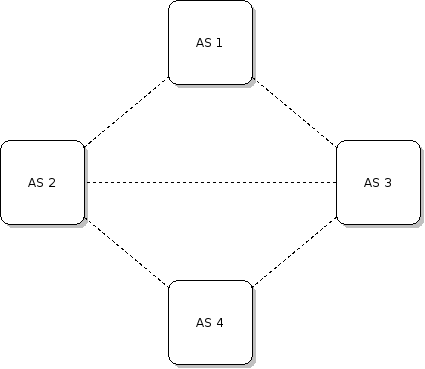
\includegraphics[width=70mm,keepaspectratio=true]{./figures/BGP_iranyitatlan.png}\hspace{5mm}
    % BGP_iranyitatlan.png: 425x369 pixel, 72dpi, 14.99x13.02 cm, bb=0 0 425 369
    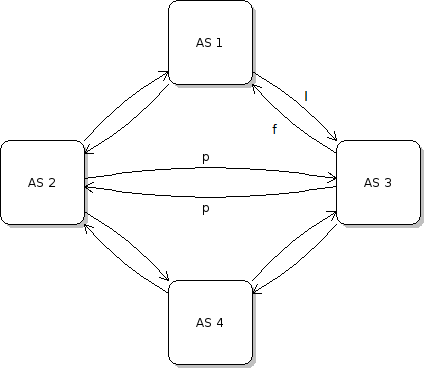
\includegraphics[width=70mm,keepaspectratio=true]{./figures/BGP_iranyitott_labeled.png}
    % BGP_iranyitott_labeled.png: 425x369 pixel, 72dpi, 14.99x13.02 cm, bb=0 0 425 369

    \caption{A BGP egyszerűsített képe és a völgymentesség szerinti irányítás.}
    \label{fig:figure_BGP}
  \end{figure}

  Érdemes megvizsgálni a BGP szabályrendszerét: a BGP routing policy-ja többszintű. A legalsó szint, a legalapvetőbb policy a völgymentesség. Ez azt jelenti, hogy az útvonalválasztásnál elsődleges szempont, hogy semelyik AS-nek ne kelljen fizetni olyan forgalomért, ami csak áthalad rajta. Ha a hierarchiában lefelé mutató éleket $l$-lel, a felfelé mutató éleket $f$-fel, a peering kapcsolatokat pedig $p$-vel jelöljük, akkor minden routing során kijelölt útvonal csak a következő alakban írható le: néhány (akár nulla) $f$ él, aztán maximum egy $p$ él, utána pedig néhány (akár nulla) $l$ él.\\

  Emellett, ha felhasználjuk a gráfbeágyazás és kompakt routing eredményeit, akkor egy új távolságfüggvénnyel és a csomópontok koordinátázásával megvalósítható az Internet tartományszintű gráfjában is egy elakadásmentes mohó útvonalválasztás \cite{DobreiBScSzakdolgozat}.

  \begin{figure}[h]
    \centering
    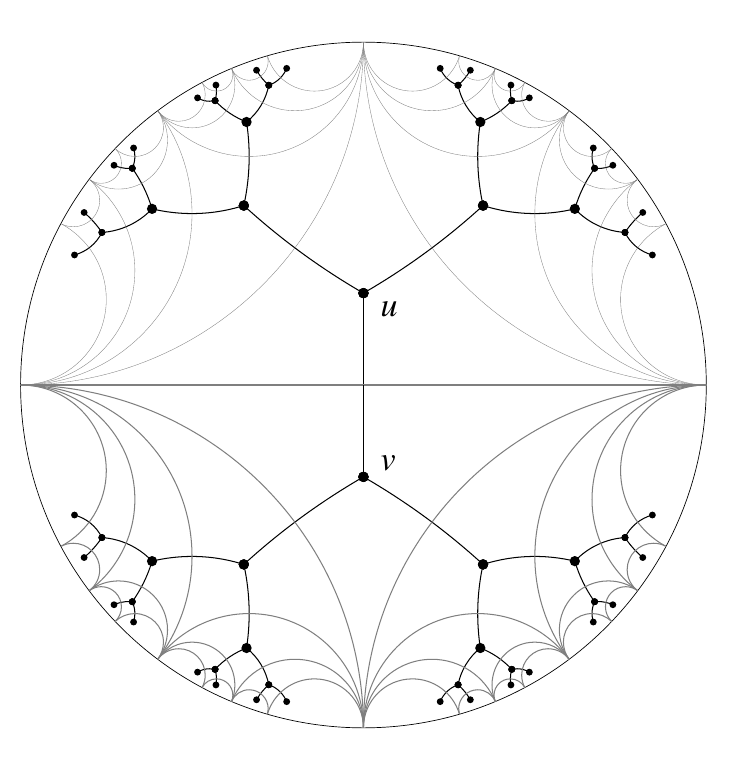
\includegraphics[width=70mm]{./figures/3-reg_disk.png}\hspace{5mm}
    % 3-reg_disk.png: 749x757 pixel, 96dpi, 19.81x20.03 cm, bb=0 0 562 568
    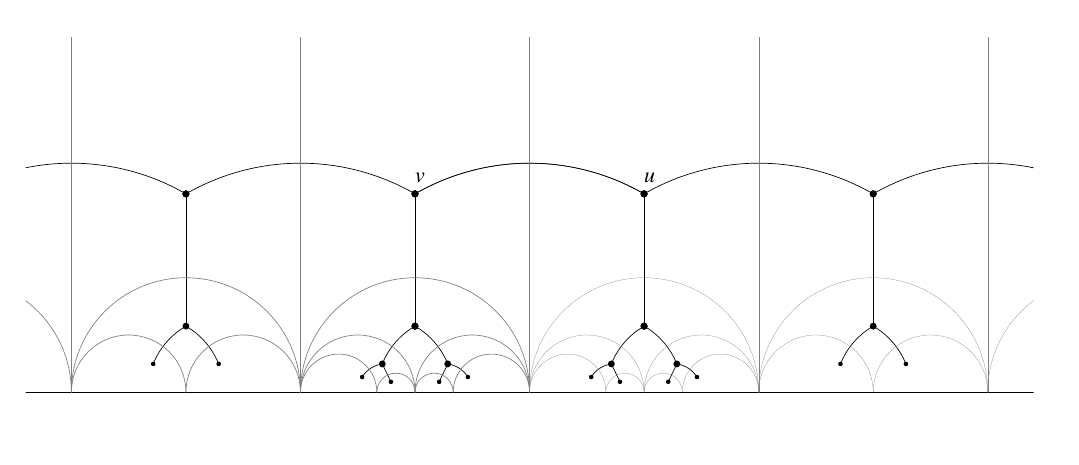
\includegraphics[width=70mm,keepaspectratio=true]{./figures/3-reg_half_plane.png}
    % 3-reg_half_plane.png: 1079x465 pixel, 96dpi, 28.54x12.30 cm, bb=0 0 809 349

    \caption{A hiperbolikus sík Poincaré-féle diszk modellje és a felső félsík modellje \cite{Klein07}.}
    \label{fig:figure_hiperbolikusabrak}
  \end{figure}

  A $\mathbb{H}$ hiperbolikus síknak többféle szemléltető modellje is van, ám a két legelterjedtebb a felső félsík modell és a Poincaré diszk modell, amiket \aref{fig:figure_hiperbolikusabrak} ábrán láthatunk is. A Poincaré modellben $\mathbb{H}$-t egy egységkörrel reprezentálják: $x^2~+~y^2~<~1$, a következő metrikával:
  \begin{align}
    ds^2~=~\frac{4(dx^2~+~dy^2)}{(1~-~x^2~-~y^2)^2}.
  \end{align}

  A felső félsík modellben $\mathbb{H}$-t a $\{\langle x,y\rangle ~|~y~>~0\}$ ponthalmaz írja le, ahol a metrika:

  \begin{align}
    ds^2~=~\frac{dx^2~+~dy^2}{y^2}.
  \end{align}

  Mindkét esetben a $\mathbb{H}$ pontjait komplex számokként kezeljük: $(x,y)~\in~\mathbb{R}^2:~z~=~x~+~yi$.

  Ezek alapján két új policy-t mutatok be:

  \begin{itemize}
    \item Hiperbolikus-távolság: Az elakadásmentes mohó útvonalválasztás policy-ja.
    \item Völgymentesség: A BGP alapvető, elsődleges policy-ja.
  \end{itemize}

      %----------------------------------------------------------------------------
      \subsubsection{Hiperbolikus-távolság}
      %----------------------------------------------------------------------------

      A hiperbolikus síkra ágyazott Internet gráf minden pontja egy $(x,y)$ koordinátapárral leírható. A policy algebrája a $\mathcal{H}$ ($\mathbb{R}^{+},~\infty,~f_{\mathbb{H}},~\leq$), ahol $f_{\mathbb{H}}$ egy viszonylag bonyolult függvény, definiálásához szükséges lenne több, itt nem részletezett ismeret a hiperbolikus geometria témaköréből (bővebben ld. \cite{Thurston97} 2. fejezetét).

      %----------------------------------------------------------------------------
      \subsubsection{Völgymentesség}
      %----------------------------------------------------------------------------

      A völgymentesség policy-nak az algebrája a $\mathcal{V}$ ($\{f,~l,~p\},\phi,\bigoplus_{\mathcal{V}},\preceq$),  ahol a $\bigoplus_{\mathcal{V}}$ \aref{tab:szumma_tab} táblázat szerinti\footnote{ Egy adott súlyú (típusú) úthoz hozzá akarnánk venni egy élet, akkor az út milyen súlyúvá (típusúvá) válna.}. Az előbbi szabály másik megfogalmazásban azt jelenti, hogy sem $l$-t, sem $p$-t nem követhet sem $p$, sem $f$.

      \begin{table}[ht]
        \footnotesize
        \centering
        \caption{A $\bigoplus_{\mathcal{V}}$ \cite{Compact_Policy_Routing}.}
        \begin{tabular}{ c | c c c }
          $\bigoplus$ & $f$ & $l$ & $p$\\
          \hline
          $f$ & $f$ & $l$ & $p$\\
          $l$ & $\phi$ & $l$ & $\phi$\\
          $p$ & $\phi$ & $p$ & $\phi$\\
        \end{tabular}\label{tab:szumma_tab}
      \end{table}\newpage

  %----------------------------------------------------------------------------
  \section{Egyéb algebrák}
  %----------------------------------------------------------------------------

  A minél részletesebb vizsgálat érdekében definiálok olyan policy-kat is, melyek vagy minden eddigi modellben használható lenne, vagy egyikben sem, így eddig nem volt lehetőségem bemutatni.

  A fejezet legelején felvázolt két dimenzió (optimalizálás, érdekek) mellett a harmadik karakterizálási lehetőség az időbeli lefolyás. Ha egy útvonalválasztási probléma tárgyalása során figyelembe vesszük az időt is, mint befolyásoló tényezőt, egy olyan új dimenziót ragadunk meg, mely minden modell routing-ját képes befolyásolni: ez az \emph{Időfüggés} policy. A vírus-terjedésnél elég csak arra gondolni, hogy télen könnyebben tud terjedni a fertőzés, és hasonlóan nyáron nagyobb valószínűséggel terjed egy fürdőruhadivat. Fontos azonban, hogy ez csak egy mellékes faktor, azaz egy alap policy mellett van értelme figyelembe venni az időpontot is. Az Internetes útvonalválasztás során időfüggést tapasztalhatunk, ha pl. egy terheléselosztó rendszer egy adott kérést másodpercenként váltakozva egyszer kiszolgál, egyszer pedig újrapróbálkozásra szólít fel.\\

  Másik érdekes policy, a trendterjedésnél említett leghosszabb út policy. Ennek olyan esetben van értelme, amikor nem a célba érkezés a legfontosabb, hanem maga az út. A vírus- és trendterjedésnél ez azért volt lényeges, hogy minél több embert elérjünk, de pl. a hangyák is így építik ki a bolyban az utakat, hogy egy esetleges betolakodó minél nagyobb valószínűséggel eltévedjen.

      %----------------------------------------------------------------------------
      \subsubsection{Leghosszabb-út}
      %----------------------------------------------------------------------------

      A leghosszabb-út policy adja az elérhető leghosszabb utat. Ebben az esetben az $\mathcal{L}$ algebra az $(1, 0,~+,~\geq)$ négyes. Ebben a policy-ban minden él konstans 1 súlyú, egy út súlya éppen az élszáma.

      %----------------------------------------------------------------------------
      \subsubsection{Időfüggés}
      %----------------------------------------------------------------------------
      Az Időfüggés policy lényege, hogy az időpontot\footnote{A lépték mértéke problémafüggő: lehet naponkénti éves periódusokkal, lehet } figyelembe véve néha átjárhatatlan egy-egy él. Ehhez szükséges egy alap policy is, amelyet ez ki tud egészíteni: $\mathcal{A}$. Jelölje $T_{e_i}$ az időpontok egy olyan halmazát, melyben $\mathcal{I}$ nem enged át forgalmat az $e_i$ élen. (A $T_{e_i}$ lehet akár egy $[t_0, \infty)$ intervallum is.) Így az $\mathcal{I}$ algebra: $(W_{\mathcal{A}},~\phi_{\mathcal{A}},~f,~\preceq_{\mathcal{A}})$, ahol
      $$f(e_1,e_2,t)~=~
      \begin{cases}
        \phi_{\mathcal{A}} & \text{ha } t \in T_{e_1} \cup T_{e_2}\\
        e_1 \bigoplus_{\mathcal{A}} e_2 & \text{különben}
      \end{cases}$$

      Azaz, alkalmas időpontban teljes egészében az $\mathcal{A}$ policy érvényesül, azonban minden élen bizonyos időpontokban nem lehet átmenni.\\

  %----------------------------------------------------------------------------
  \section{Összefoglaló}
  %----------------------------------------------------------------------------
  Ebben a fejezetben megvizsgáltam a hálózatkutatás szempontjából alapvető modelleket, melyeket a lokális- vagy globális optimalizálás és a közös- vagy egyéni érdekek követése tulajdonságok alapján karakterizáltam. Bemutattam a fertőző betegségek vizsgálatára használt matematikai modellt, megvizsgáltam a témakör útvonalválasztási kérdéseit és kijelöltem a két, a problémakört jól jellemző policy-t: a Fertőzési-határ és az Unió-fedés policy-ket, illetve ezek algebráit: $\mathcal{F}$ = ($(0,1],~0,~max,~\geq$) és $\mathcal{U}$ = ($\mathbb{N},~\infty,~f,~\leq$).

  Rávilágított a trend- és a vírusterjedés hasonlóságaira és különbségeire útvonalválasztási szempontból és definiáltam két policy-t, a Összekötő-keresés-t és a Korai-elfogadó-keresés-t. Ezen policy-k algebrái: $\mathcal{O}$ = ($(1,d),~0,~max,~\geq$) és $\mathcal{K}$ = ($\mathbb{N},~-1,~+,~\geq$).

  Végül megvizsgáltam a már ismertetett policy-kon (ld. \aref{section_algebrapeldak}. alfejezetet) kívül az Internet tartományszintű gráfjának az alapszabályát, a Völgymentességet, illetve felvázoltam a hiperbolikus térbe ágyazás - általa pedig az elakadásmentes mohó útvonalválasztás - lehetőségét: $\mathcal{V}$ = ($\{f,~l,~p\},\phi,\bigoplus_{\mathcal{V}},\preceq$) és $\mathcal{H}$ = ($\mathbb{R}^{+},~\infty,~f_{\mathbb{H}},~\leq$).

%----------------------------------------------------------------------------
%\Aref{framework}. fejezetben az előző vizsgálatok alapján egy olyan modellezési keretrendszer dolgozok ki és mutatok be, melynek segítségével a nagyméretű valós hálózatokat jellemző útvonalkialakítási dinamikát vagyok képes strukturált módon jellemezni.
%----------------------------------------------------------------------------
\chapter{A modellezési keretrendszer}\label{framework}
%----------------------------------------------------------------------------
\Aref{examples}. fejezetben bemutattam, hogy hogyan lehet az ott ismertetett problémák vizsgálatára hasznosítani a routing algebrák matematikai modelljét. Ahhoz, hogy ezt a gyakorlatban is fel tudjuk használni, az algebrákat szoftveresen is felhasználható módon kell leírni. Emellett ki kell dolgozni azt a modellezési, szimulációs eljárást is, amely keretrendszerként képes a változatos bemeneteket kezelve elemezni a különböző útvonalválasztási szabályrendszerek felderítését.\\

Ezt a keretrendszert ebben a részben mutatom be. \Aref{section_specification}. rész elején pontosítom, hogy mit lehet elvárni egy ilyen rendszertől. Részletezem az adatok előzetes feldolgozására, tisztítására vonatkozó elvárásokat, melynek során kitérek a feladat domainének esetleges szűkítésére is. Kijelölöm a szimulációtól elvárt működést és definiálom, hogy milyen kimenete legyen a rendszernek.\\
Ezután \aref{section_simulator}. részben a keretrendszer egy konkrét megvalósítását írom le, melynek részeként ismertetem az algebrák implementálást, elemzem a felhasznált útvonalválasztó (optimalizáló) algoritmust. Ezután bemutatom, hogy hogyan értékelem ki a szimulációs eredményeket, hogyan hasonlítom össze az eredetileg választott (megfigyelt) útvonalakat a policy primitívek által adott utakkal.\\
Végül \aref{section_real}. részben bemutatom, hogy egy valós hálózatot (repülési adatok alapján) hogyan lehet vizsgálni az itt ismertetett keretrendszer segítségével.

  %----------------------------------------------------------------------------
  \section{Specifikáció}\label{section_specification}
  %----------------------------------------------------------------------------
  Ahogy a szoftvertermékeknél általában, ebben az esetben is meghatározó, hogy milyen specifikációnak kell megfelelnie a modellezési keretrendszernek. Ehhez természetesen meg kell határozni, hogy milyen célokat szeretnék elérni és ha erre szükség van, azt is, hogy hogyan szeretnénk céljainkat elérni.\\

  A keretrendszer fő célja, hogy a routing algebrák felhasználásával elemezni és akár visszafejteni is képesek legyünk kívülről megfigyelt útvonalválasztási szabályrendszereket. Ehhez alapvető, hogy a keretrendszer megfelelő rugalmassággal tudja használni az algebrákat, a definiált algebrák műveleteit képes legyen használni, valamint tudja az algebrákon értelmezett műveleteket is kezelni. Emellett szükség van egy általános formátumra is, melyre a bemeneti adatokat át tudjuk konvertálni. Az ebben a formátumban lévő adathalmazon értelmezni kell egy optimalizáló függvényt, mely az adott algebrák rendező operátora ($\preceq$) alapján kiválasztja utak egy halmazának leginkább preferált útjait.

    %----------------------------------------------------------------------------
    \subsection{A formátum}
    %----------------------------------------------------------------------------
    Mivel szeretnénk minél több problémát vizsgálni a rendszer segítségével, pontosítani kell, hogy milyen az elvárt bemenet. Le kell képezni az általános problémát egy jól strukturált, könnyen kezelhető modellre. Ahogy ezt már bemutattam \aref{section_routingalgebrak}. részben, erre kiválóan alkalmas egy irányított, súlyozott teljes gráf. Ennek a gráfnak az élsúlyai többdimenziós vektorok, amelyeknek minden egyes komponense egy-egy (probléma-specifikus) tulajdonságként értelmezett súlyt tartalmaznak.

      %----------------------------------------------------------------------------
      \subsubsection{Az adatok előfeldolgozása, tisztítása}\label{prep}
      %----------------------------------------------------------------------------
      Ahhoz, hogy az irányított, súlyozott teljes gráfban értelmezni tudjuk az adott problémát, mindenképpen szükség van szakterület-specifikus tudásra, azaz a problémakör ismeretére. Ezt azért nem tudjuk automatizálni, mert sokszor a rendelkezésre álló adatok nem az egyes kapcsolatokhoz vannak rendelve, hanem például a csomópontokhoz. Ezeket a speciális eseteket le kell fordítani élsúlyozásra. Emellett természetesen lehetséges, hogy maga a problémakör olyan információkat is kezel, amelyekre nincs szükségünk. Ebben az esetben ezen adatokat ki kell szűrni, amihez szintén szakterület-specifikus tudásra van szükség.\\

      A gráf csúcshalmazát viszonylag egyszerűen meg tudjuk határozni, hiszen általában a problémakörök esetében tudjuk, hogy milyen csomópontokat értelmezünk. Az élhalmaz esetében már nem ilyen egyértelmű a helyzet, de ha nem tudunk jó becslést adni, értelmezhetjük a teljes gráfot, mint bemenetet. Ez természetesen igen költséges lehet mind tárkapacitásban, mind algoritmikus futási időben. Ezért lehet szükséges az élhalmaz csökkentése, azaz az útvonalválasztási szabályrendszer domainének szűkítése. A Pareto-elv\footnote{A Pareto-elv, más néven a 80/20 szabály kimondja, hogy számos jelenség esetén a következmények 80\%-a az okok mindössze 20\%-ára vezethető vissza.} értelmében megpróbálhatjuk az élek egy részét kizárni a vizsgálatból, azaz törölni, vagy az algebra $\phi$ elemével súlyozni. (A végtelennel súlyozáskor természetesen az él megmarad, de az adott algebra biztosan nem fogja használni, ami az optimalizáló algoritmus futását gyorsíthatja, valamint fontos megemlíteni, hogy élet csak olyan esetben tudunk törölni, ha egyik algebra sem használná.)\\

      A bemenet értelmezése során tehát az igazán fontos feladat az élek súlyának és irányításának meghatározása. Mivel nagy hálózatok vizsgálásakor a gráf gyorsan kezelhetetlen méretűvé válhat, ezért mindig a vizsgálni kívánt algebráknak megfelelően érdemes a súlyozást és az irányítást elvégezni. Például ha egy algebra $\preceq$ operátora egészeket \textit{hatékonyabban} tud összehasonlítani, mint valósokat, emellett a tényleges súlyok nagyságrendje miatt elhanyagolható a törtrész, akkor érdemes a (pontos-, de akár lekerekítéssel képzett) egész részekkel dolgozni.

      %----------------------------------------------------------------------------
      \subsection{Az optimalizálás függvénye}
      %----------------------------------------------------------------------------
      Miután legeneráltuk az irányított, vektor-súlyozott gráfot, szükség van egy függvényre, mely ki tudja választani utak egy halmazának legjobb útjait. Ezen legjobb utak algebránként változnak, ám az algoritmus lehet ugyanaz. Ilyen a következő algoritmus:

      \begin{algorithm}
        \caption{Optimalizáló függvény}\label{algo_optimalizalo}
        \begin{algorithmic}[1]
          \Procedure{getPreferredPath}{$Vertex~u,~Vertex~v,~Algebra~a$}
            \State $\textit{paths} \gets \Call{getAllPathsBetween}{u,~v}$
            \State $\textit{preferred} \gets [~]$

            \For{\textbf{each} \textit{path} in \textit{paths}}
              \If {$a_W(path_i)~a_\preceq~a_W(path)$}
                \State $\textit{preferred} \gets \textit{preferred}~+~path$
              \EndIf
            \EndFor
          \EndProcedure
        \end{algorithmic}
      \end{algorithm}

      Természetesen ez a függvény nem implementálható ebben a formában, hiszen nincs részletezve, hogy hogyan működik a $\Call{getAllPathsBetween}{u,~v}$, de az általános felhasználhatósága látszódik az 5. sorban: az összes út közül a legjobbakat kiválasztani csupán az aktuális algebra alapján is képesek vagyunk. (Itt jól látszik egy algebra ,,jól viselkedése'', hiszen a $\Call{getAllPathsBetween}$ függvény akár a gráf méretében exponenciális méretű úthalmazzal is visszatérhet.)\\

      A konkrét implementálás előtt gondoljuk meg, hogy érdemes az összes út előállítása, majd a minimálisak kiválasztása helyett csak a minimális utak megtalálását megpróbálni. Egy minimális út keresésére számtalan \textit{mohó} megoldás ismert, melyek optimálisak és a gráf méretéhez képest polinom időben futnak. Nem triviális probléma azonban az \textit{összes} ilyen út megtalálása. Erre a problémára használható egy módosított Dijkstra algoritmus, melyet a Függelékben részletezek (lásd \aref{dijkstra}. rész).

    %----------------------------------------------------------------------------
    \subsection{A kimenet}
    %----------------------------------------------------------------------------
    A szimulációs folyamat kimenetelén statisztikai elemzéseket szeretnénk lefolytatni, ezért ügyelni kell arra, hogy ez biztosítva legyen, illetve a folyamat lefutása közbeni értékes adatokat is gyűjteni, menteni és a kimeneten pedig feltüntetni szükséges.\newpage

  %----------------------------------------------------------------------------
  \section{A szimulátor}\label{section_simulator}
  %----------------------------------------------------------------------------
  A szimulációs algoritmus a fent leírt irányított, súlyozott gráfon, mint bemeneten fut. Először meghatározzuk, hogy a konkrét probléma vizsgálata mekkora csúcshalmazt jelent, amelyből előáll egy $G(V=n, E=n \cdot (n-1))$ méretű gráf\footnote{Minden csúcsot minden csúccsal összekötünk és mindkét irányban irányítunk.}. Ezután meghatározzuk azon éleket, melyet ezen a gráfon az útvonalválasztási szabályrendszer akármilyen két pont között legalább egyszer használt. Ezt természetesen meg tudjuk tenni, hiszen a kialakult utakat megfigyelni képesek vagyunk. Miután meghatároztuk a felhasznált élhalmazt, minden olyan élet, amelyet nem tartalmaz ez a halmaz kitörlünk a gráfból (Az élek törlésével nem eshet szét a gráf, hiszen a ponthalmazt megfigyeléssel kaptuk, így biztos, hogy összefüggő marad a gráf.). A megmaradó éleket súlyozzuk.\\

  A szimuláció menete ezután a következő: Minden pontpárra és minden vizsgált algebrára meghatározzuk (a módosított Dijkstra algoritmussal), hogy milyen ut(ak)at jelölnek ki. Az így meghatározott ut(ak)at feljegyezzük. Ezzel előállítunk két gráfot: az első az eredetileg vizsgált gráf, a másik a feljegyzett utakból felépülő. Ezután ezen két gráfot hasonlítjuk össze.

    %----------------------------------------------------------------------------
    \subsection{A matematikai struktúrák implementálása}
    %----------------------------------------------------------------------------
    A különböző matematikai struktúrák felhasználása nem magától értetődő. Mivel bármilyen útvonalválasztási szabályt el lehet képzelni, és viszonylag egyszerűen meg lehet alkotni az ehhez tartozó algebrát, nem mindig egyszerű megfogalmazni a számítógép nyelvén ezeket.\\
    Ahhoz, hogy a módosított Dijkstra algoritmus futtatható legyen, négy alapvető funkcióval kell ellátni egy ,,szoftver-algebrát'': Egy súlyfüggvénnyel (\texttt{W(Route route)}), egy összegző függvénnyel (\texttt{bigOPlus(Weight w1, Weight w2)}), egy átjárhatatlanságot (végtelen súlyt) jelentő függvénnyel (\texttt{phi()}) és egy olyan függvénnyel, amely megadja, hogy szerinte mi a legjobb (legkisebb) súly (\texttt{best()}). Látszódik, hogy a matematikai struktúra nem ültethető át tisztán egy szoftverbe, nincs szükség például a súlyok alaphalmazára, ez nem az algebrához tartozik egy szimulátoron belül (persze ismerni kell a halmazt).\\

    A másik absztrakt fogalom, amit a szimuláció során használok, az a gráf, csúcsaival és éleivel. Mivel itt a csúcsoknak már biztosan nem tulajdonítunk semmilyen információhordozó szerepet (lásd a csúcsok adataink élekre való átírását \aref{prep}. szakaszban), egy egyszerű (egész) azonosítóval jelöljük, míg az élek -- összetettségük miatt -- már bonyolultabb modellt igényelnek, melyek azonban mindig az adott problémától függenek és algebra-súly párokat tartalmaznak (adott algebra szerint mi a súlya az élnek).\\
    A gráfot ezután vagy éllistával, vagy szomszédossági mátrixszal jeleníthetjük meg. A szomszédossági mátrix a sűrű gráfoknál hatékonyabb, de az itt vizsgált problémák általában ritka gráfokkal modellezhetők\footnote{Ha elfogadjuk, hogy \textit{valamilyen} elv szerint optimális az útvonalválasztás, akkor nem lehet sok párhuzamos út $u$ és $v$ között, hiszen a redundancia nem hatékony az élszámok tekintetében.}. Mégis a módosított Dijkstra algoritmust a mátrixos megadásra készítettem fel pusztán a programozástechnikai egyszerűsége miatt (természetesen a mátrixos megadásnak az optimalizált formáját használom, azaz csak a létező éleknél tárolok adatot).

    %----------------------------------------------------------------------------
    \subsection{A felhasznált algoritmus elemzése}
    %----------------------------------------------------------------------------

                \todo

  %----------------------------------------------------------------------------
  \section{A szimulációs eredmények kiértékelése}
  %----------------------------------------------------------------------------
  A szimulációs folyamat két gráfot eredményez, melyek összehasonításával szeretnénk meghatározni, hogy az adott algebra mennyire képes leírni az eredeti (csupán megfigyelt) útvonalválasztási szabályrendszert.

    %----------------------------------------------------------------------------
    \subsection{A vizsgálandó metrikák}
    %----------------------------------------------------------------------------
    A két gráfot -- az eredetit és a generáltat -- szeretnénk összehasonlítani, hogy mennyire hasonlítanak. A pontos egyezés eldöntése általában nehéz feladat, hiszen a gráfok izomorfiájának\footnote{Két gráf izomorfiáján bijektív struktúratartó leképezést értünk, lásd pontos definíciót \aref{grafizo} résznél.} eldöntése ugyan NP-beli (bővebben lásd \aref{eldontesi_def}. definíciót), de nem ismert hatékony módszer rá. Emellett nyílván az is szempont, hogy itt az is fontos és használható eredmény, ha nagyon hasonlítanak egymásra a gráfok (hálózatok), mert ez azt jelentené, hogy a nem ismert útvonalválasztási szabályt jól tudtuk becsülni az adott algebrával. Ez abban az esetben érdekes, ha az eredeti szabályrendszer bonyolult, vagy pl. egy mesterséges hálózat esetén nem automatizált: ekkor ugyanis a bonyolult szabályrendszert le lehet cserélni a szimuláció során használt policy primitív(ek)re. Így tehát még abban az esetben sem lenne érdemes izomorfiát vizsgálni, ha rendelkezésünkre állna egy erre alkalmas algoritmus.\\

    Kétféle szempontrendszer szerint hasonlítom össze a gráfot: pontpáronként és globális hálózati mutatók alapján. Alapvető különbség van a két megközelítésben, hiszen különböző tulajdonságokat lehet megtudni a kétféle vizsgálatból.\\

    A pontpárok közötti összehasonlítása során megvizsgálom, hogy a megfigyelt és a szimulált út mennyire hasonlít a lépésszám és az érintett köztes csomópontok alapján és ez alapján inkább jobb vagy inkább rosszabb a szimulált út, esetleg nem eldönthető (ez mindig függ a problémától, ezért a kiértékelésnél is szükség van probléma-specifikus tudásra).\\

    A globális hálózati metrikák közül a fokszámeloszlást fogom vizsgálni, valamint az élek számát, a hálózat átmérőjét és az élösszefüggőségét. A fokszámeloszlás és az átmérő összehasonlításra azért van szükség, mert ezek alapvető karakterisztikáját adják a hálózatnak. Ezzel feltárhatók olyan változások, melyek a pont-pont kapcsolatok vizsgálata során nem vettünk észre, például lehetséges, hogy a valóságban skálafüggetlen hálózatnak a fokszámeloszlása a szimuláció során már sokkal kiegyensúlyozottabb lesz. Hasonlóan fontos az élösszefüggőség, mellyel a gyakorlati használhatóságot mérhetjük, hiszen az eredetinél a szétesésre jóval érzékenyebb gráf esetén nem érdekes, hogy a többi szempont szerint ,,jól teljesít'' az adott algebra.\\

    Minden fent említett összehasonlítási szempontot pontozok a következő részekben meghatározottak szerint és így minden szimulációs eredményt (algebrát) egy pontszámmal fogok tudni mérni, melyben a több a jobb, így könnyen meg tudom mondani, hogy az algebrák hogyan teljesítenek egymáshoz képest. A szempontoknál jellemzően háromféle pont adható: a legtöbb pont arra jár, ha szimulált eredmény a megfigyelttel megegyezik, ennél kicsivel kevesebb pontot ér, ha az adott szempont szerint jobb, illetve a legkevesebb (akár negatív pont is lehetséges), ha rosszabb annál.\\

    Ahhoz, hogy meg tudjuk mondani, hogy milyen pontszám az, ami már elég pontosnak számít, referencia szimulációkat futtatok. Egy ilyen referencia vizsgálat során tudom, hogy milyen útvonalválasztási szabályrendszer alakította ki az utakat a hálózatban, így tudom, hogy egy adott algebrának hogyan kéne teljesítenie. Ezután az ezen a gráfon futtatott szimulációs eredményeket ki tudom értékelni, így megkapom azt a pontértéktartományt, illetve küszöbértéket, ami felett elfogadhatóan pontosnak tartok egy algebrát.\\
    A következőkben leírt pontértékeket egy kezdeti pontozásból kiindulva a referencia szimulációk során finomhangolva határoztam meg. Emellett külön figyelmet fordítottam arra, hogy különböző mérőszámokat különböző súllyal szeretnék figyelembe venni.

    %---------------------------------------------------------------------------
    \subsubsection{Az algebra szerinti távolság pontozása}
    %----------------------------------------------------------------------------
    Az algebra szerinti távolságot pontértékét $AL$-lel jelölöm ($AL$: $A$lgebra$L$ength). Az $AL$ értékét úgy alakítom ki, hogy nagy hangsúlyt kapjon, hiszen ez az a tulajdonság, ami miatt az algebrákkal foglalkozom, amit le tudnak írni a policy-kból a matematika nyelvén. Ezért a pontosan becsült út 10 pontot, a rövidebb út 8 pontot, míg a megfigyeltnél hosszabb út 3 pontot jelent. Mivel minden pontpárra vonatkozik a pontozás, ezért egy $n$ csúcsú gráf esetén a $3n \leq AL \leq 10n$.

    \begin{note}
      Ha a megfigyelt hálózatban csak az összes útvonalat ismerjük és ebből egy élhalmazt kapunk meg, akkor természetesen nem triviális, hogy hogyan kezeljük az algebra szerinti távolságot, sőt a következő pontpárokra értelmezett pontokat sem. Nem tudjuk biztosan megmondani, hogy az élhalmazból melyik élek mentén jutunk el a pontpárok között. Abban az esetben viszont, ha a megfigyelés úgy történik, hogy az adott pontpárok közötti utakat ismerjük (figyeljük meg), akkor nincs ilyen probléma.
    \end{note}

    %----------------------------------------------------------------------------
    \subsubsection{A lépésszám szerinti távolság pontozása}
    %----------------------------------------------------------------------------
    Hasonlóan az $AL$ pontozáshoz, a lépésszám szerinti távolság pontértékét a $HC$ ($H$op$C$ount) jelöli. Ez a mutató jóval inkább mennyiség, mint minőségi mutató, hiszen az algebra alapvető hozzáadott értékét (a speciális távolságmérést) figyelmen kívül hagyja, nem törődik a meghatározott út távolságával, csak nagyon áttételesen. Ezért a pontértékek rendre 5, 4 és 1 pont. Egy algebra és egy $n$ csúcsú gráf esetén $1n \leq HC \leq 5n$, így mondhatjuk, hogy egy adott út lépésszámának pontos szimulációja legfeljebb kétharmad annyit ér, mint az algebra szerinti távolsága pontos szimulációja.

    %----------------------------------------------------------------------------
    %\subsubsection{Az út során érintett köztes csomópontok pontozása}
    %----------------------------------------------------------------------------
    %A két csomópont közti út során érintett csúcsok pontértékét az $IV$ ($I$nside$V$ertices) jelöli. Ez a mutató algebra függő, mert vannak olyan problémák, ahol teljesen lényegtelen, hogy milyen csomópontokon halad végig az út, máshol viszont ez magát az útvonalválasztást befolyásoló tényező. Az algebrafüggésből adódóan itt a három eset (pontos, jobb, rosszabb) további pontosításra szorul\footnote{Ezt mindig az aktuális vizsgálatnál kell megtenni, lásd \aref{test}. fejezetet.}, a pontértékük rendre 5, 4 és 1 pont, hasonlóan a $HC$ mutatóhoz.

    %----------------------------------------------------------------------------
    \subsubsection{A fokszámeloszlás pontozása}
    %----------------------------------------------------------------------------
    A fokszámeloszlás már globális mutató, melyet $DD$-vel ($D$egree$D$istribution) jelölök. Ez a tulajdonság olyan alapvető, hogy nem különböztetek meg ,,pontos'', jobb és rosszabb esetet, csak \textit{hasonló}t és \textit{különböző}t, melyek pontértéke rendre 1 és 0. A $DD$ mutatót nem is összegezve számítom bele a végpontszámba, hanem szorzótényezőként, így az, hogy hasonlítson a szimulált hálózat fokszámeloszlása a megfigyeltéhez egy szükséges feltétele annak, hogy értékelhető megoldást kapjunk. Ezutén a $DD$ értéke a következő:

    $$ DD = \left\{
    \begin{array}{l l}
      1 & \quad \text{ha megegyezik a fokszámeloszlás}\\
      0 & \quad \text{különben}
    \end{array} \right.$$

    Mivel a fokszámeloszlás egy hisztogram, nincs értelme pontos egyezőséget vizsgálni, de több jó módszer is létezik két hisztogram összehasonlítására. Ilyen módszer a $\chi^2$ távolság mérése.

    \TODO{histogram}

    %----------------------------------------------------------------------------
    \subsubsection{A hálózat-átmérő pontozása}
    %----------------------------------------------------------------------------
    A hálózat átmérője azért ad fontos információt, mert az átmérő a hálózat tömörségét mutatja, azaz azt, hogy maximálisan mennyi lépést kell megtenni a gráfban, ha tetszőleges két pont között akarunk útvonalat választani. Ha nagy az átmérő, az tipikusan azt jelenti, hogy könnyen lehet alternatív utakat találni, hiszen ezeket még nem találták meg, használták fel. Hasonlóan olyan hálózatokban, amelyek tömörek, az átmérőjük kicsit, nehéz ,,jó'' alternatívákat keresni, hiszen -- legalábbis a hop-szám tekintetében -- csupa rövid út köti össze a pontpárokat. Emellett fontos megjegyezni, hogy az átmérő csak más hálózati mutatókkal együtt hordoz értelmezhető jelentést.\\
    Ennek fényében a $GD$ ($G$raph$D$iameter) jelölésű pontérték megegyezik a hálózat tényleges átmérőjével.

    %----------------------------------------------------------------------------
    \subsubsection{Az élösszefüggőség pontozása}\label{elossze}
    %----------------------------------------------------------------------------
    Egy gráf pont- illetve élösszefüggősége kiszámítható legfeljebb $\binom{n}{2}$ maximális folyam keresésével. Nagamochi és Ibaraki megmutatta, hogy a probléma megoldására elegendő $O(mn)$ idő is\cite{Nagamochi96}. A pontösszefüggőségi számot $\kappa(G)$-vel, az élösszefüggőségi számot pedig $\lambda(G)$-vel jelölve felírhatjuk azt az egyszerű észrevételt, miszerint legalább annyi élet kéne elhagyni a gráf széteséséhez, mint pontot: $\kappa(G) \leq \lambda(G)$ azaz egy $k$ pontösszefüggőségből következik a legalább $k$ élösszefüggőség. Emellett fontos megjegyezni, hogy a szimulációs eredmények kiértékelése folyamán a pontösszefüggőséget nem fogom külön vizsgálni, mert a legtöbb probléma vagy úgy áll elő, vagy olyan alakra transzformálható, ahol nem lehet értelmezni egy csomópont törlését. Természetesen azon speciális esetekben, ahol ez nem így van és tényleges jelentést is hordoz a $\kappa(G)$, ott ezt a mutatót is érdemes vizsgálni.\\

    Mivel az élösszefüggőséget könnyen el lehet torzítani, nem tisztán a $\lambda(G)$-t határozom meg. A valóságban megfigyelhető hálózatok túlnyomó többsége skálafüggetlen, és mint olyan, sok alacsony fokszámú csúcsot tartalmaz, jellemzőn elsőfokúakat is, amikor $\lambda(G)$ = 1, de a gráf ,,mag''-járól, annak tömörségéről nem ad információt. Ezért a $C$ (Edge$C$onnectivity) pontérték a csomópontok fokszámeloszlás szerinti felső 20\%-nak minimális fokszáma lesz. Ez megegyezik ezen 20\% élösszefüggőségével, hiszen az a csomópont, aminek pontosan ennyi a fokszáma, egy ekkora vágással eltávolítható a gráfból.

    %----------------------------------------------------------------------------
    \subsubsection{Az élszám pontozása}
    %----------------------------------------------------------------------------
    Az élszám pontozását $EC$-vel ($E$dge$C$ount) jelölöm. A $EC$ olyan a $DD$-nek, mint a $HC$ az $AL$-nek, azaz a hasonló típusú mutatók közül ez inkább a mennyiségi, a $DD$ a minőségi mutató. Éppen ezért kevesebb értékkel, jelentéssel bír az $EC$. Ha pontosan ugyanannyi élet használ a szimulált gráf, mint a megfigyelt, akkor $EC$ = $an + b$ (a csúcsszámmal lineáris a kapcsolat, jellemzően n/20), ha nem, akkor $EC~=~f(C)$, azaz függ az összefüggőségtől, méghozzá úgy, hogy
    $$0 > \frac{\partial EC}{\partial C}$$
    Ez azt jelenti, hogy az élösszefüggőség pontértékének növekedésével csökken az élszám pontértéke. Erre azért van szükség, mert az élösszefüggőség magas értékéből következik a magas élszám, és ugyanazt a jelenséget (sok él van a gráfban) nem szeretnénk duplán értékelni.

    %----------------------------------------------------------------------------
    \subsubsection{A globális mutatók egymásra hatása, együttes értékük}
    %----------------------------------------------------------------------------
    Az összes globális mutatóról elmondható, hogy tényleges értéket, értelmezhető jelentést csak akkor hordoznak, ha egymással kapcsolatban vannak értelmezve, mégpedig a megfelelő hatásokat és ellenhatásokat figyelembevéve. A $GV$ ($G$lobal$V$alue) értéket a következő összefüggések befolyásolják:
    $$0 < \frac{\partial GV}{\partial GD}$$
    $$0 < \frac{\partial GV}{\partial C}$$
    $$0 > \frac{\partial GV}{\partial EC}$$
    Egy ilyen függvény a következő:
    $$GV = \frac{DD \cdot GD \cdot C}{EC}$$

  %----------------------------------------------------------------------------
  \section{Valós hálózatok vizsgálata a keretrendszer segítségével}\label{section_real}
  %----------------------------------------------------------------------------
  Mivel a diplomamunka feladatkiírásában nem volt benne, hogy saját szimulátort kell használnom, az ezzel kapcsolatos technikai részletek a Függelékben (\aref{simulator}. rész) található.\\

  \Aref{examples}. fejezetben definiált algebrák modellezése után valós hálózatokon vizsgálhatjuk a viselkedésüket, hogy hogyan alakítanak ki utakat. Ezután tetszőleges algebrák lexikografikus szorzatát is szimulálhatjuk, így még pontosabb és változatosabb modellt kapunk.


  %----------------------------------------------------------------------------
  \section{Összefoglaló}
  %----------------------------------------------------------------------------
  Ebben a fejezetben leírtam egy olyan keretrendszert, melynek segítségével szimulálás segítségével össze lehet hasonlítani különböző algebrákat ugyanazon a problémán. Specifikáltam ezt a rendszert, felvázoltam az elvárt célokat. Ezután leírtam az általános problémák előfeldolgozását, a tisztított és előkészített adatok alapján a szimuláció pontos menetét. Meghatároztam a szempontokat, ami alapján a szimulációs eredményeket értékelni lehet, ehhez pedig kidolgoztam egy pontrendszer, mely figyelembe veszi, hogy az elsődleges cél a megfigyelt útvonalválasztási szabályok visszafejtése, így a pontozásban a helyesen megtalált utak érik a legtöbbet, utána következnek az eredetinél jobb utak és legutoljára az eredeti rosszabb utak.\\
  A pontrendszer kidolgozását referencia szimulációk futtatásával támogattam, melynek segítségével már nem csak az algebrákat tudom összehasonlítani egymással, hanem egy abszolút mércét is kaptam.

%----------------------------------------------------------------------------
\chapter{�sszefoglal�s}\label{sect:chapter_test}
%----------------------------------------------------------------------------

%----------------------------------------------------------------------------
\chapter{Összefoglalás}\label{summary}
%----------------------------------------------------------------------------
A feladatkiírás pontjainak eleget tettem. A szakirodalom alapján a hálózatkutatás eredményeit áttekintettem, különös tekintettel az útvonalválasztás matematikai kérdésére. Megvizsgáltam több különböző, valós életből származó hálózati útvonalválasztással szoros kapcsolatban álló problémakört, és mindegyik ilyenhez definiáltam útvonalválasztási stratégiákat, melyek vizsgálata új megvilágításba helyezné ezeket a problémákat. Specifikáltam egy szimulációs keretrendszert, mellyel lehetőség nyílik az új stratégiák vizsgálatára. Egy ilyen vizsgálatot el is végeztem, amely során a repülőtársaságok útvonalválasztását vizsgáltam meg.\\

\Aref{modell}. fejezetben áttekintettem a szakirodalmat, összeszedve a legfontosabb állomásokat. Rámutattam, hogy az Internet AS-szintű topológiáján kívül, a más tudományterületekről származó problémák útvonalválasztásáról sem tudunk sok mindent. Ezért szükséges egy olyan eszköz, ami a policy-feltárás feladatát -- általános esetben is -- hatékonyan el tudja látni. Ehhez definiáltam a \textit{routing algebrákat}, bemutattam a legfontosabb tulajdonságait és műveleteit, emellett a legszélesebb körben használt policy-k algebráit is ismertettem.\\

\Aref{examples}. fejezetben megvizsgáltam és legfontosabb tulajdonságaik alapján karakterizáltam a hálózatkutatás szempontjából alapvető modelleket. Bemutattam a fertőző betegségek vizsgálatára használt matematikai modellt, megvizsgáltam a témakör útvonalválasztási kérdéseit és kijelöltem a két, a problémakört jól jellemző policy-t. Emellett rávilágított a trend- és a vírusterjedés útvonalválasztási szempontbeli hasonlóságaira és különbségeire is és definiáltam két új trendterjedési policy-t. Megvizsgáltam az Internet tartományszintű gráfjának a szabályrendszerét, a völgymentességet, illetve felvázoltam a hiperbolikus térbe ágyazás -- általa pedig az elakadásmentes mohó útvonalválasztás -- lehetőségét.\\

\Aref{framework}. fejezetben specifikáltam és megterveztem egy szimulációs keretrendszert, mellyel valós hálózati problémákon lehet tesztelni különböző útvonalválasztási stratégiák alapján leírt algebrákat. Definiáltam a szimulációhoz szükséges előfeldolgozási, adattisztítási lépéseket és magát a szimulációs folyamatot. Emellett kidolgoztam egy pontrendszert, mellyel értékelni lehet a szimulációs eredményeket. Referencia szimulációkkal úgy alakítottam ki ezt a pontrendszert, hogy ne csak egy relatív skálát kapjak, ahol csak a vizsgált algebrákat hasonlíthatom össze egymással, hanem egy abszolút mércét is jelentsen az eredmény pontértéke.\\

\Aref{test}. fejezetben bemutattam a vizsgálandó valós hálózatot. Az adatok feldolgozása után meghatároztam a vizsgálandó hálózatot. Definiáltam a vizsgálandó metrikákat, amik mentén össze tudtam hasonlítani a valós- és a policy vezérelt útvonalválasztás által meghatározott útvonalakat és hálózatokat. Minden pontpárra megvizsgálta, az eredeti és a szimulált út különbségeit (távolság, lépésszám). A valós és a szimulált hálózatok statisztikai összehasonlítását is elvégeztem, melyben figyelmet fordítottam a fokszámeloszlás, a hálózatok átmérőjének és az élösszefüggőségének összehasonlítására.\\

A saját magam írt szoftverrel futtatott szimulációk eredményeinek alapján kijelenthető, hogy a diplomamunkámban tárgyalt keretrendszer -- megfelelő körülmények között -- alkalmas valós hálózati útvonalválasztási problémák vizsgálatára, algebrák tesztelésére.


\listoffigures\addcontentsline{toc}{chapter}{Ábrák jegyzéke}
%\listoftables\addcontentsline{toc}{chapter}{Táblázatok jegyzéke}

\bibliography{content/mybib}{}
\addcontentsline{toc}{chapter}{Irodalomjegyzék}
\bibliographystyle{my_bibtex_style}
%%----------------------------------------------------------------------------
% A bibtex m�g nem megy, addig is, j� lesz ez...
%----------------------------------------------------------------------------

\begin{thebibliography}{9}\addcontentsline{toc}{chapter}{Irodalomjegyz�k}

\bibitem{DuncanWatts} Duncan J. Watts, \emph {Networks, Dynamics, and the Small-World Phenomenom}.
American Journal of Sociology, Volume 105, Issue 2, 493-527. oldal, 1999.

\bibitem{DobreiMScOnlab1} D�brei G�bor, \emph {Nagym�ret� h�l�zatok evol�ci�ja - Trendterjed�s vizsg�lata szimul�ci�s eszk�z�kkel}.
Besz�mol�, BME TMIT, H�l�zatok �s szolg�ltat�sok, �n�ll� laborat�rium 1., 2013.


%----------------------------- introduction -----------------------------


\bibitem{Heuristics_for_Internet_Map_Discovery} Ramesh Govindan, Hongsuda Tangmunarunkit, \emph {Heuristics for Internet Map Discovery}.
INFOCOM 2000. Nineteenth Annual Joint Conference of the IEEE Computer and Communications Societies. Proceedings. IEEE Volume 3, 1371-1380. oldal, 2000.

\bibitem{Inferring_AS_level_Internet_Topology_from_Router_Level_Path_Traces} Hyunseok Chang, Sugih Jamin, Walter Willinger, \emph {Inferring AS-level Internet Topology from Router-Level Path Traces}.
In Proceedings of SPIE ITCom 2001, 2001.

\bibitem{On_Inferring_and_Characterizing_Internet_Routing_Policies} Feng Wang, \emph {On Inferring and Characterizing Internet Routing Policies}.
Proceeding IMC '03 Proceedings of the 3rd ACM SIGCOMM conference on Internet measurement, 15-26. oldal, 2003.

\bibitem{The_Impact_of_Routing_Policy_on_Internet_Paths} Hongsuda Tangmunarunkit, Ramesh Govindan, Scott Shenker, Deborah Estrin, \emph {The Impact of Routing Policy on Internet Paths}.
INFOCOM 2001. Twentieth Annual Joint Conference of the IEEE Computer and Communications Societies. Proceedings. IEEE Volume 2, 736-742. oldal, 2001.

\bibitem{Sobrinho_Algebra_and_Algorithms} J. L. Sobrinho, \emph {Algebra and Algorithms for QoS Path Computation and hop-by-hop Routing in the Internet}.
IEEE/ACM Transactions on Networking (TON), Volume 10., Issue 4, 541-550. oldal, 2002.

\bibitem{Compact_Policy_Routing} R�tv�ri G., Guly�s A., Heszberger Z., Csernai M., Bir� J., \emph {Compact Policy Routing}.
Proceedings of the ACM Principles of Distributed Computing, 2011.

\bibitem{Sobrinho_Network_routing} J. L. Sobrinho, \emph {Network routing with path vector protocols: theory and applications}.
In SIGCOMM '03, 49-60. oldal, 2003.

\bibitem{Sobrinho_Metarouting} T. Griffin, J. L. Sobrinho, \emph {Metarouting}.
SIGCOMM '05, 1-12. oldal, 2005.

\bibitem{Lexicographic_products_in_metarouting} A. Gurney, T. Griffin, \emph {Lexicographic products in metarouting}.
In Network Protocols, IEEE International Conference on, 113-122. oldal, 2007.

\bibitem{Quality_of_service_routing_for_supporting_multimedia_applications} Zheng Wang, Jon Crowcroft, \emph {Quality-of-service routing for supporting multimedia applications}.
IEEE Journal of Selected Areas in Communications, Volume 14, Issue 7, 1228-1234. oldal, 1996.

\bibitem{Quality_of_service_based_routing_A_performance_perspective} G. Apostolopoulos, R. Guerin, S. Kamat, S. K. Tripathi, \emph {Quality of service based routing: A performance perspective}.
In SIGCOMM, 17-28. oldal, 1998.

\bibitem{On_path_selection_for_traffic_with_bandwidth_guarantees} Qingming Ma, P. Steenkiste, \emph {On path selection for traffic with bandwidth guarantees}.
In Proceedings of the 1997 International Conference on Network Protocols (ICNP '97), 191. oldal, 1997.

%----------------------------- chatper 1. -----------------------------

\bibitem{Lamport94} Leslie Lamport , \emph {\LaTeX : A Document Preparation System}.
Addison Wesley, Massachusetts, 2nd Edition, 1994.

\bibitem{Amport94} Amport , \emph {\LaTeX : A Document Preparation System}.
Addison Wesley, Massachusetts, 2nd Edition, 1994.

\end{thebibliography}

%----------------------------------------------------------------------------
\appendix
%----------------------------------------------------------------------------
\chapter*{F�ggel�k}\addcontentsline{toc}{chapter}{F�ggel�k}
\setcounter{chapter}{6}  % a fofejezet-szamlalo az angol ABC 6. betuje (F) lesz
\setcounter{equation}{0} % a fofejezet-szamlalo az angol ABC 6. betuje (F) lesz
\numberwithin{equation}{section}
\numberwithin{figure}{section}
\numberwithin{lstlisting}{section}
%\numberwithin{tabular}{section}

%----------------------------------------------------------------------------
\section{A TeXnicCenter fel�lete}
%----------------------------------------------------------------------------
\begin{figure}[!ht]
\centering
\includegraphics[width=150mm, keepaspectratio]{figures/TeXnicCenter.png}
\caption{A TeXnicCenter Windows alap� \LaTeX-szerkeszt�.} 
\end{figure}

%----------------------------------------------------------------------------
\clearpage\section{V�lasz az ,,�let, a vil�gmindens�g, meg minden'' k�rd�s�re}
%----------------------------------------------------------------------------
A Pitagorasz-t�telb�l levezetve
\begin{align}
c^2=a^2+b^2=42.
\end{align}
A Faraday-indukci�s t�rv�nyb�l levezetve
\begin{align}
\rot E=-\frac{dB}{dt}\hspace{1cm}\longrightarrow \hspace{1cm}
U_i=\oint\limits_\mathbf{L}{\mathbf{E}\mathbf{dl}}=-\frac{d}{dt}\int\limits_A{\mathbf{B}\mathbf{da}}=42.
\end{align}







\label{page:last}
\end{document}
























































 